\documentclass[draft=false,oneside]{fduthesis}
\usepackage{booktabs}
\usepackage{graphicx}
\usepackage{subcaption} % 用于子图
\usepackage{float} % 控制图像位置
\usepackage{listings}

\fdusetup{
    style = {
        font-size = 5,
        fullwidth-stop = false,
        logo = fig/logo1.png,
        auto-make-cover = true
    },
    info = {
        title = {深度学习在单分子荧光定位显微镜中的应用},
        title* = {Deep learning in Single Molecule Localization Microscopy},
        author = {凌星皓},
        supervisor = {张云翔},
        major = {化学(强基计划)},
        department = {化学系},
        student-id = {21307110019},
        school-id = {10246},
        keywords = {单分子成像,单分子定位荧光显微镜,深度学习,编码-解码网络,像差矫正},
        keywords* = {Single-molecule imaging, Single-molecule localization microscopy, Deep learning, Encoder-decoder, Aberration correction},
        secret-level = {none},
    }
}

\begin{document}

    \tableofcontents

    \begin{abstract}
        面对较厚生物组织中单分子成像面临的随视野变化的像差问题，本文使用标量衍射理论对三维的点源扩散函数和像差进行了建模，同时可模拟相位掩膜以生成如双螺旋形的三维点源扩散函数。使用波前相位差描述失焦带来的影响，并加入散粒、泊松、读出噪声，由此生成随机点源的单分子模拟图像。为了去除随视野变化而随机扰动的波前像差，使用含有13阶随机Zernike像差(0.65rad rms)的不同密度的随机点源图像作为训练集，不含像差和噪声的理想图像作为标注数据，搭建了基于编码-解码器的有监督卷积神经网络以矫正像差。矫正后的图像表现出更好的质量，并在定位精度测试中优于未矫正图像。
    \end{abstract}

    \begin{abstract*}
        The field-of-view dependent aberration in single molecule imaging in deep tissue samples causes degraded resolution and localization precision. In this work, simulation based on scalar diffraction theory is built to generate 3D point spread function: a phase mask could be incorporated to generate double helix PSF or other engineered PSF; defocus is incorporated into pupil function by wavefront analysis; the 2D image of randomly distributed bulrred points in 3D space are then calculated and different kinds of noise are simulated. Then, random coefficients of Zernike aberrations is also incorporated into the pupil function to account for the wavefront aberration caused by deep tissue. The above serving as training set, an encoder-decoder convolutional network is constructed to compensate for the aberration to get a clean, noise-and-aberration-free image. The effect of the network is shown and a localization accuracy test is performed to see an improvement brought by the network.
    \end{abstract*}

    \chapter{引言}

    \section{单分子定位显微成像技术}
    \par 随着物质科学的发展进入微观时代，为了克服传统宽场成像受衍射极限(diffraction limit)制约的痛点，研究者们开拓了以单分子中心的一系列新技术。其中，单分子定位显微镜(Single Molecule Localization Microscopy)是一种基于单个发光分子精确定位的成像技术，常用于超分辨成像(Superresolution Imaging)和单粒子追踪(single molecule tracking)技术中。前者以随机光学重建显微镜(Stochastic Optical Reconstruction Microscope)\cite{rustSubdiffractionlimitImagingStochastic2006}为代表，利用多次少量激活的密标记荧光分子重建超越衍射极限分辨率的图像。后者则通过若干单分子的时间追迹，获得生物体内分子的扩散、转运等动力学信息。这两种技术的实现都依赖于对单个荧光分子的准确定位。
    
    \par 概括来说，单分子定位是一个逆问题：未知位置的单个点源经过成像系统所采集得到的信号称为点源扩散函数(point spread function, PSF)。多个点源的信号以非相干(incoherent)的方式线形相加即得到最终的图像。算法的目标即通过获得的图像反推点源的位置、亮度等参数。然而由于背景、光子、传感器噪声的存在，信号应理解为一个随机变量，因而需要设计拟合所得信号。理想情况下，焦面上的点源扩散函数可证明为一个艾里斑(Airy Partten)，其详细导出见第二章。在大多数情况下可以进一步近似为一个高斯函数。流行的软件包(ThunderSTORM )\cite{ovesnyThunderSTORMComprehensiveImageJ2014}提供质心法、拟合法和最大似然估计法以求得单分子坐标。其算法一般流程包括坐标矫正、背景扣除、局部最大值的识别分割、计算单分子坐标等步骤，见图\ref{trd}。

    \begin{figure}[h] 
        \centering
        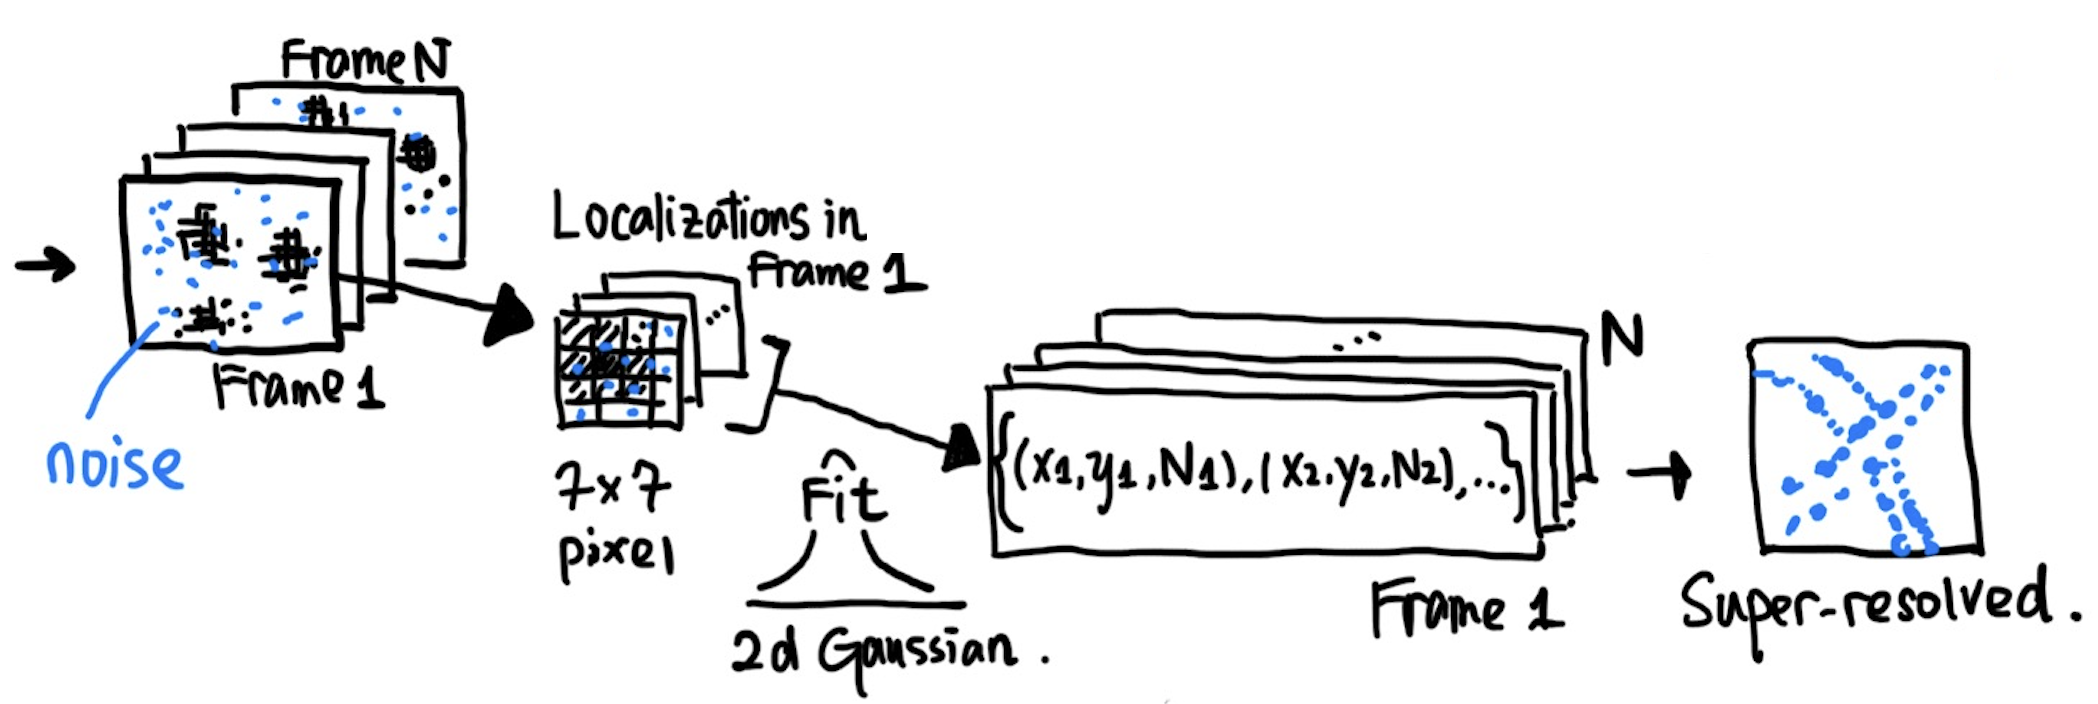
\includegraphics[width=0.7\textwidth]{fig/software.png}
        \caption{传统单分子定位流程示意图}
        \label{trd}
    \end{figure}

    \par 然而，许多因素会导致其信号并非理想的艾里斑，从而令上述拟合流程失效。一方面，快速成像可能会需要高密度的激发、或低的曝光时间。由此导致的信号混叠和信噪比降低会显著影响拟合的准确性。另一方面，离焦误差、脱离显微镜本身矫正的位置、介质折射率的不匹配、生物体内复杂的环境则会引入复杂的像差，尤其是在进行组织内深度的成像时。这对单分子追踪和超分辨成像都是不利的，尤其是三维的单分子定位。此外，PSF工程(PSF Engineering)则通过在傅立叶面上进行相位调制(如使用可变形镜和液晶空间相位调制器)以人为改变PSF形状，使单个点源能更好的编码z轴等信息。显然，这也对新兴的定位算法提出了挑战。


    \section{PSF重建和像差矫正方法研究现状}

    精确的PSF为各类定位算法提供了基础，因而值得仔细的讨论。一般而言，在二维定位问题中，镜头公差(tolerance)级别的像差不会对传统高斯函数拟合的定位精度造成很大的影响\cite{stallingaAccuracyGaussianPoint2010}。但在更高维度的定位问题和较大像差存在时(如生物组织)，其对PSF对影响不可忽略。基于标量衍射理论的分析使我们可通过光瞳函数的傅里叶变换“从头计算”PSF\cite{goodmanIntroductionFourierOptics2005}和3D PSF\cite{mccutchenGeneralizedApertureThreeDimensional1964}。显微镜成像系统可以直接借助数值孔径(Numerical Aperture, N.A.)和介质的折射率使用这套计算方法。而另一方面，每一台显微镜和具体的成像条件会导致多种偏离理想的PSF，导致这种简单计算与实际不相符。

    \par 因而，自然的想法是通过细致的建模精细化成像模型。为了矫正介质不匹配(玻璃、油、生物组织之间)导致的球差(spherical aberration)\footnote{球差是一种低阶像差，可理解为多项式展开的前部项，详见第二章的讨论}，Gibson-Lanni模型\cite{gibsonExperimentalTestAnalytical1991}使用几何光学和衍射理论给出修正的光程差。矢量模型\cite{torokElectromagneticDiffractionLight1997}则考虑到荧光偶极子发射的极化特点，这一点在高N.A.的系统中更加明显。然而，生物组织(如细胞器)含有折射率各不相同的一系列部件，其波前畸变的方式一般无法用简单的球差来描述。

    \par 通常来说更方便的策略是对荧光微珠进行不同焦面的成像(beads calibration)以实验地获得3D的PSF。对获得的z图像堆进行三次条样插值(cspline interpolatation)\cite{liRealtime3DSinglemolecule2018}即可得到便于快速计算的3D PSF。但是，该方案只能对某一z区间的微珠进行标定。尽管有研究通过整合Gibson-Lanni模型\cite{mcgortyCorrectionDepthdependentAberrations2014}来计算深层的PSF，这对于复杂、变动的组织中成像仍然是不现实的。

    \par 折中的方法源于标量/矢量模型的拓展。简单来说，像差可以描述为与理想情况下波前(例如一个汇聚的球面波)的偏离，从而折算在一个单一的光瞳函数(pupil function)中。通过测量点光源在不同离焦程度下的图样，可以对光瞳函数进行迭代更新，直到修正的光瞳函数可以还原出与实验相近的3D PSF。其关键算法称为相位恢复算法(phase retrieval)\cite{hanserPhaseRetrievalHighnumericalaperture2003,hanserPhaseretrievedPupilFunctions2004}，最早用于天文领域，现已有研究者将其用于单分子实验中\cite{liuThreeDimensionalSingle2013}，包括无需微珠标定的体内相位恢复\cite{xuThreedimensionalNanoscopyWhole2020}。该方法的优势在于能兼容Gibson-Lanni模型或矢量模型的修正，对深层点源的PSF计算更准确；且由于基于物理模型计算，相较插值法能够还原高频的细节。然而，迭代计算和参数优化比较耗时；在无标定的情况下依赖于对荧光分子的3D PSF的采样率，因而在实时活体成像上仍有改进空间。有研究利用神经网络(见下一节描述)对单分子荧光的发射模式进行分析\cite{zhangAnalyzingComplexSinglemolecule2018}，具有快速精确分析波前像差的潜力。
    
    \par 自适应光学(Adaptive Optics, AO)是另一种矫正像差的思路，其亦起源于天文领域，通过实时对波前进行调制，补偿由于大气扰动造成的波前像差。近来，研究者也将这项技术应用于生物成像中。如Siemons等人成功使用REALM实现对高至1 rad RMS的波前像差的矫正并用于微管的成像\cite{siemonsRobustAdaptiveOptics2021}。然而，鉴于AO体系的搭建复杂昂贵，且波前调制的分辨率有限、有延迟，其不太可能成为单分子实验的标准配置。
    
    \par 总结来说，各类重建PSF的方法各有优劣，但都难以在非标记的组织内成像场景下运作，更无法实时对画面进行矫正；基于自适应光学的方案具有实时矫正的优点，但配置复杂、难以普及。

    \section{机器学习技术在单分子成像中的应用}
    \par 机器学习(machine learning)可以理解为一种令程序“自动”分析数据从而“掌握”数据中隐含的规律的算法，已被广泛用于信号处理、数据分析、自然语言处理等领域。其中，基于卷积神经网络(Convolutional neural networks, CNN)的方法以被成功应用于图像识别、生物图像分区、单帧分辨率提升等问题中。近年来，研究者发展出一系列基于机器学习的方法以改善1.1节中提到的成像问题。得益于图像处理单元(graphic processing unit)和计算能力及的提升，其中大部分方法的计算速度能够超越传统的优化方法，为定位算法提供了新的视角。
    \par 针对高密度的定位场景，Shechtman课题组率先发展了基于深度卷积网络的二维定位算法DeepSTORM\cite{nehmeDeepSTORMSuperresolutionSinglemolecule2018}。考虑到点源数量的不确定性，使用高分辨的网格(grid)作为神经网络的输出，以编码解码(encoder-decoder)结构作为网络架构，而后再用简单的算法定位每个分子的位置。其训练集由物理模型或实验(稀疏已定位的亮点源的多帧叠加)得到。该方法相较传统方法在高密度数据集的分析和计算速度上有较大优势。几乎同时，Boyd等人亦通过卷积神经网络DeepLoco实现了三维的单分子定位\cite{boydDeepLocoFast3D2018}。其关键区别在于后者直接以单分子的三维坐标作为网络输出、而非输出一个高分辨的网格。另一个重要区别在于使用实验测试得到的PSF作为生成训练集的模型，而非简单的高斯模型(见上一节描述)。
    \begin{figure}[h] 
        \centering
        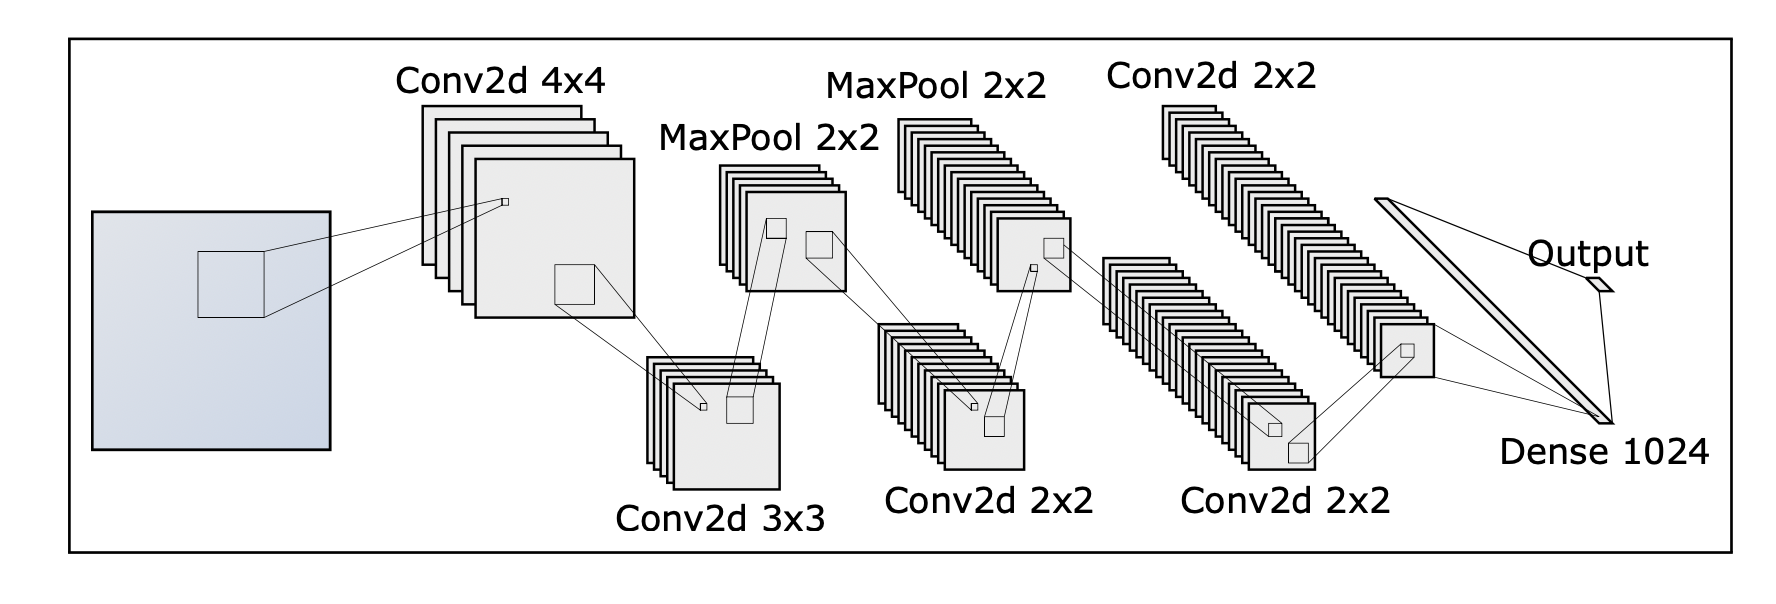
\includegraphics[width=0.7\textwidth]{fig/simpleCNN.png}
        \caption{DeepLoco网络架构}
        \label{deeploco}
    \end{figure}
    \begin{figure}[b] 
        \centering
        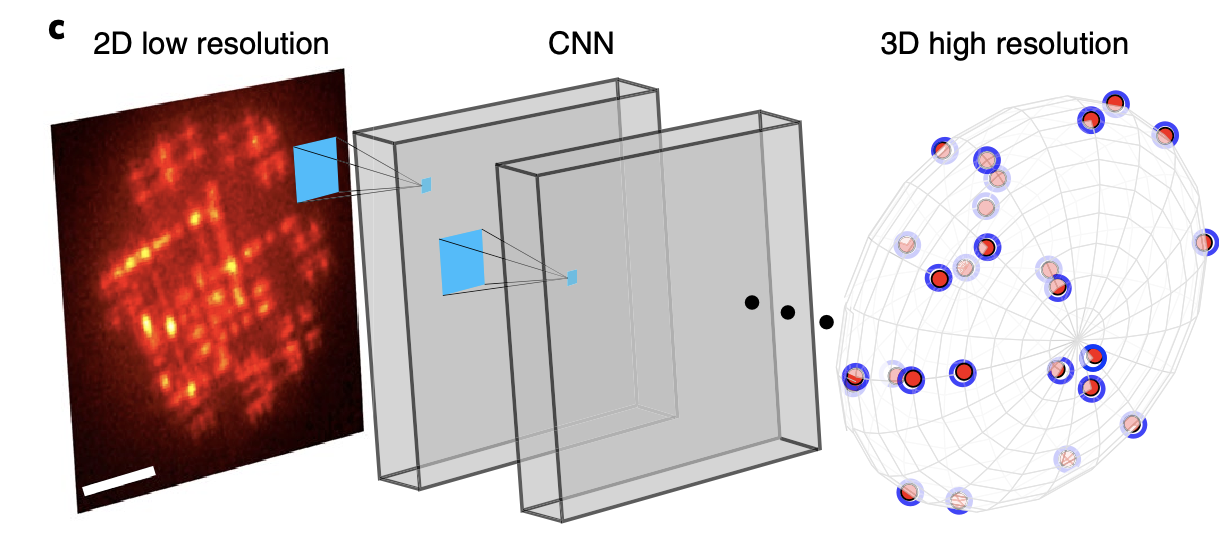
\includegraphics[width=0.7\textwidth]{fig/3DSTORM.png}
        \caption{DeepSTORM3D网络架构}
        \label{deepstorm3d}
    \end{figure}

    \par 另一方面，Zelger等人\cite{zelgerThreedimensionalLocalizationMicroscopy2018}针对稀疏的\textbf{单个点源}的三维定位发展了一种卷积网络，即需要先检测(detect)单分子点源并分割出包括一定范围周边的区域，后用模型进行精准定位(localize)。其同样以一个包含坐标、亮度、背景噪声的向量作为输出。除此外，作者还展示了准确的PSF对定位精度的影响，并使用相位恢复算法计算Zernike系数得到更精确的三维PSF。因为神经网络的输出维度对整体计算量影响较小，理论上可以训练网络输出多种信息。包括Zernike系数、取向(orientation)、多色分辨(multicolor)、流动性(mobility)等\cite{zhangUltrafastAccurateRobust2013}\cite{hershkoMulticolorLocalizationMicroscopy2019}\cite{gaireAcceleratingMulticolorSpectroscopic2020}\cite{zhangAnalyzingComplexSinglemolecule2018}。

    \par 2020年，Shechtman组进一步发展了可用于高密度的三维定位的卷积网络DeepSTORM3D\cite{nehmeDeepSTORM3DDense3D2020}。该网络仍基于高分辨网格，但将维度拓展至三维(图\ref{deepstorm3d})。该网络的优势在于能够对经过PSF工程改造的体积较大PSF进行定位，而这种PSF(如双螺旋形、四足形)通常更容易发生重叠而难以以普通的算法定位。此外，由于内嵌了物理层(physical layer)以生成PSF，研究者们得以对最佳相位掩膜(phase mask)进行优化，以达到更深的z轴定位。
   
    \par 次年，Artur Speiser等人发表了能够整合多帧信息的定位网络DECODE\cite{speiserDeepLearningEnables2021}。该网络同时输出检测概率、像素内的定位、定位的不确定度等信息，某种程度上整合了DeepSTORM和DeepLoco两类方法，并在各测试中大幅超越传统方法、表现略优于DeepSTORM3D。其中使用条样函数(spline function)拟合实测的PSF以生成训练集。有趣的是，虽然正文中未出现，但在该文的预印本中\cite{speiserTeachingDeepNeural2020}使用了一种自编码器(auto encoder)同时学习解码和编码以改善PSF模型与实际PSF的偏差。
    \begin{figure}[h] 
        \centering
        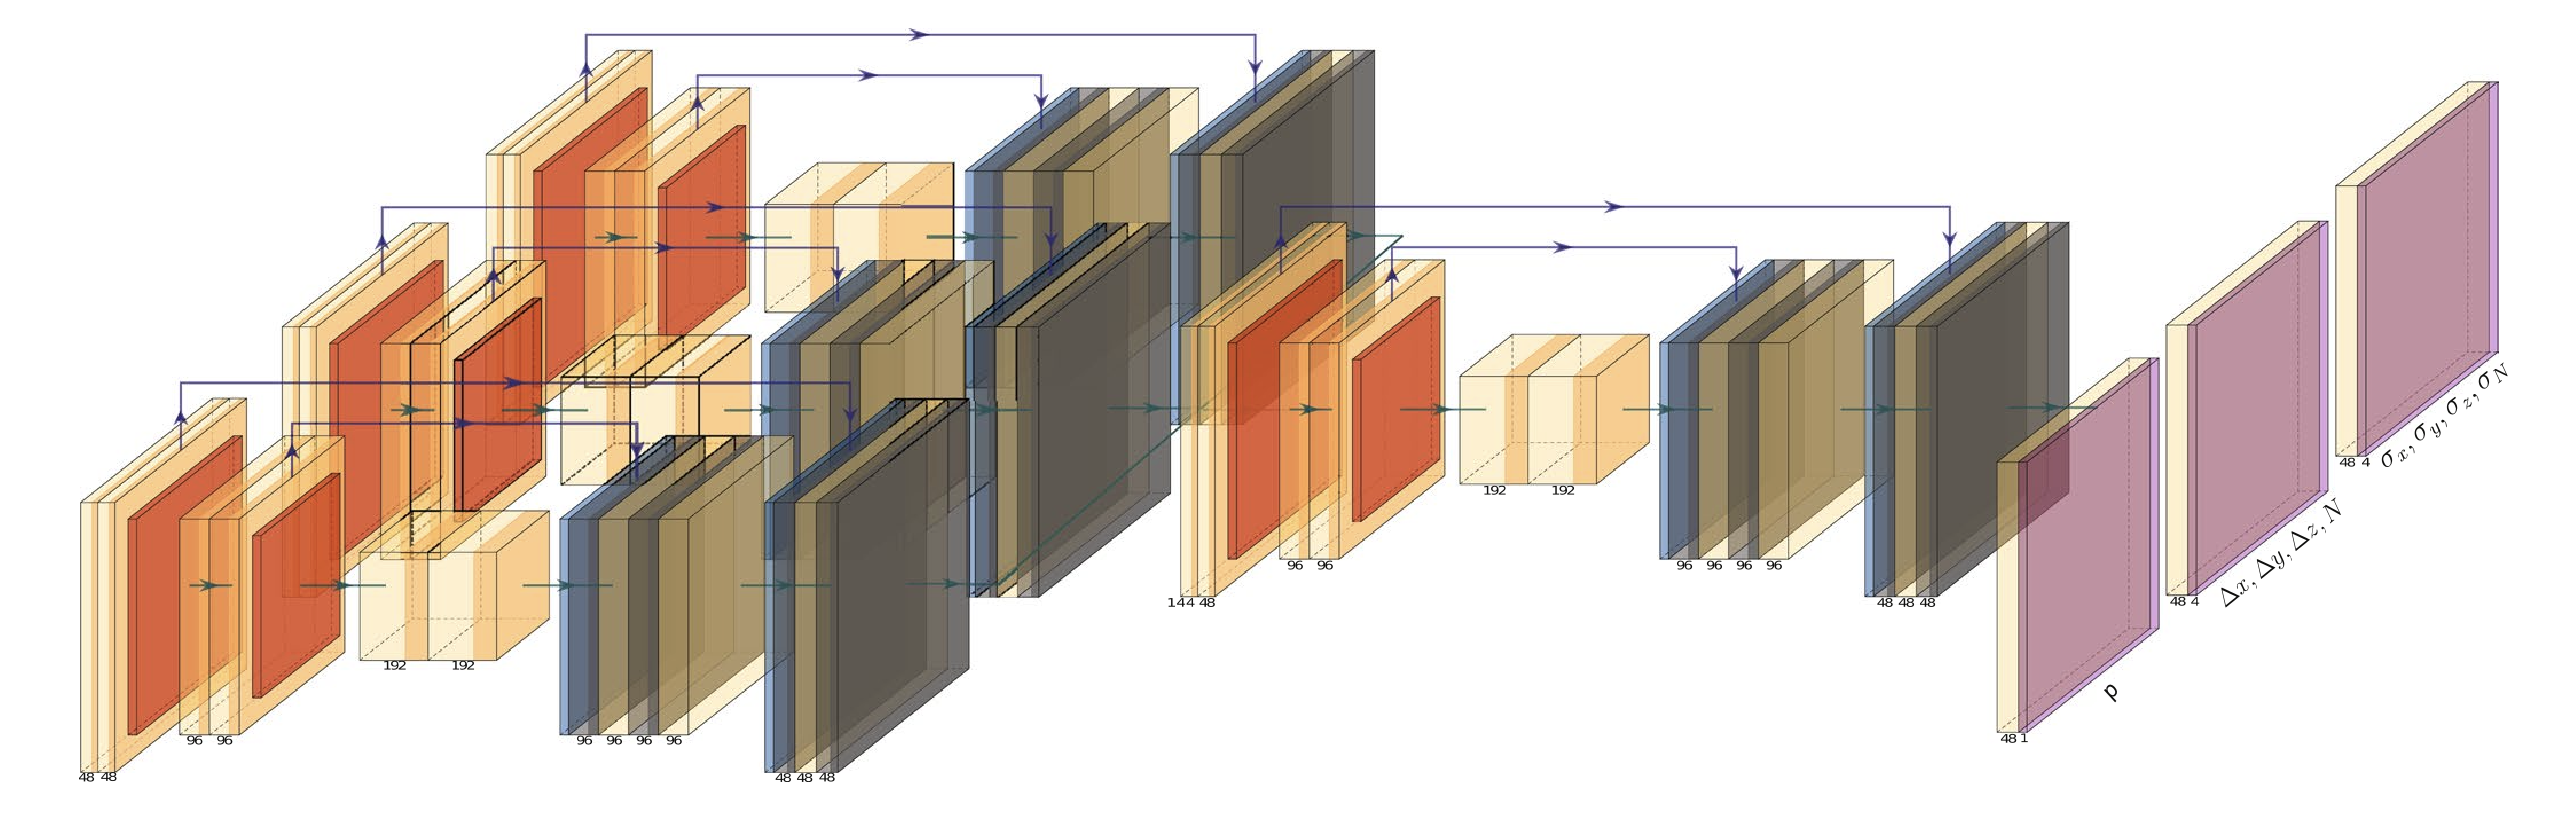
\includegraphics[width=0.7\textwidth]{fig/decode.png}
        \caption{DECODE网络架构}
        \label{decode}
    \end{figure}
    \par 最近，有研究将深度学习应用于普通荧光显微镜的深层成像中\cite{guoDeepLearningbasedAberration2025}。研究者将浅层获取的数据作为ground truth，通过添加随机的像差作为去像差网络的训练集，以实现更高分辨(如达到衍射置限水平)的深层组织成像。该方法能够达到与自适应光学相当的像差矫正能力，并可用于共聚焦、光片显微镜、多光子显微镜等多种模态。这显示出深度学习在处理去像差任务时的潜力，并提示我们可以通过令数据集尽可能遍历可能出现的各种像差以矫正快速变动和不规则的生物组织像差。

    \begin{table}[!htbp]
        \caption{机器学习算法比较} 
        \centering
        \begin{tabular}{c c c c c}
            \toprule[2pt]
            模型名字 & 网络架构 & 前/后处理 & PSF获取 & 能力\\
            \midrule 
            DeepSTORM & 编解码器 & 后续定位 & 高斯PSF & 二维定位\\
            DeepSTORM3D & 编解码器 & 后续定位 & 相位恢复 & 三维定位+PSF设计\\
            DeepLoco & CNN & 无需 & 实测PSF & 三维定位+亮度 \\
            By P.ZELGER等 & CNN & 分割点源 & 相位恢复 & 三维定位+Zernike系数等 \\
            DECODE & 多帧多通道CNN & 后续筛选 & 条样函数 & 三维检测定位+不确定性 \\
            DeAbe & 3D RCAN & 无需 & 模拟 & 像差矫正 \\
            \bottomrule [2pt]
        \end{tabular}
        \label{compare1}
    \end{table}

    \par 总结来说，机器学习的方法在单分子定位显微技术中的优势在于能够快速、高质量、多通道地分析较复杂的图像信息，从而提高快门速度、改善定位精度或提供实时的分析。其中绝大多数采用有监督学习(supervised learning)的策略，其关键步骤在于使用与实验条件匹配的模拟训练集为网络“灌注”先验的信息，如重叠PSF到坐标的映射关系、含像差图像到无像差图像到映射关系等。其中关键的选择包括：

    \begin{itemize}
        \item[1.] \textbf{网络输入} ：不同的输入具有不同的信息量。选择整张图片分析能够充分获取信息，但网络大小可能会随图片尺寸变化。而截取单分子图像快速干净，但无法应对高密度点源或复杂像差的情况。整合多帧图片能达到更高的定位精度，但也会对计算量、架构和算法提出考验。
        \item[2.] \textbf{网络输出} ：不同输出可应对不同的需求和模态。输出高分辨网格直观方便地获得高精度定位、但难以对其进行直观的评估和分析；输出点源坐标则可同传统算法直接比较，但在网络设计上较为复杂。值得注意的是多通道输出，由于神经网络的特性，能够在不增加大量运算的前提下获得更多信息，是一种可以实施的策略。
        \item[3.] \textbf{网络架构} ：网络架构主要用于解决训练的问题。深度的网络往往容易导致梯度消失、爆炸、过拟合等问题，通过设计残差网络、正则化处理可以优化这些问题。详细的讨论见第三章。
        \item[4.] \textbf{PSF获取} ：模拟的PSF同实际的PSF精准符合是提高定位精度的关键。上述算法普遍选择上一节中所述的几种方法来获得准确的PSF，需要在计算量、准确性之间做出权衡。
    \end{itemize}
    
    \section{本文的研究内容和思路}

    综上所述，目前单分子成像在存在生物组织像差的情况下，尚无成熟的定位、分析算法。而近年来基于机器学习的方法显示出其解决图像处理问题的能力。因而，本文着力于设计机器学习的架构以对含像差的单分子数据集进行快速、准确的分析，以接近自适应光学的矫正能力。具体的研究内容和路径如下：

    \begin{itemize}
    \item[1.] 建立模拟数据集。根据衍射理论，找到合理的方式生成贴合实际成像条件的3d点源扩散函数，并添加各Zernike级像差，同时模拟各类噪声。
    \item[2.] 尝试用生成的数据集训练编码解码器(encoder-decoder)、卷积神经网络(CNN)等经典深度学习模型，改进架构，验证其在模拟数据集上的像差矫正效果。
    \item[3.] 将矫正后的结果用ThunderSTORM等软件包重建坐标，比较其定位精度是否有所提高。
    \end{itemize}



    \chapter{单分子数据集的模拟}
    单分子荧光成像(single molecule fluorescence imaging)可以简述为以下过程：位于物方的荧光分子按一定的概率吸收一个激发光子，而后以一个指数分布的随机过程自发辐射(spontaneous emission)一个光子。这样而言，若激发光功率稳定，那么单分子的发射过程即可近似认为是一个柏松过程，其激发态发射概率满足：
    \begin{equation}
        \mathbb{P}\{T_{emit}>t\}=e^{-\frac{t}{\tau}}
        \label{emit}
    \end{equation}
    \par 假设不断吸收、发射光子的荧光分子具有较快的转动扩散(rotational diffusion)，那么荧光偶极子(dipole)的发射便可看作是各向同性(isotropic)且无偏振的。通常，发射光还需要经过介质（如生物膜），盖玻片，空气、水滴或油滴以进入显微镜的物镜。显微镜系统中一般则包括物镜、滤光系统、场镜，负责聚焦和选择发射光。最后，点源发出的光(近似看作发散球面波)在焦平面上成的像(汇聚的球面波)被一块图像传感器接受并转化为离散的数字信号。为了模拟单分子的信号，我们从标量衍射理论出发，逐步添加需要考虑的要素。
    \section{标量衍射理论}
    \subsection{二维点源扩散函数的导出}
    在上述过程中，点源的发射光在传播过程中被物镜的孔径限制而发生衍射。根据傅立叶光学，在标量波近似下，相干成像系统对复振幅是线形空间移不变(linear invariant system)的。像面振幅可表示为理想的几何光学锐像的复振幅场和振幅点源扩散函数$h_c$的卷积：
    \begin{equation}
        U_{img}(x,y)=U_{geo}(x,y)*h_c(x,y)=\int\int U_{geo}(x-x',y-y')h_c(x',y')dx'dy'
    \end{equation}
    其中U代表二维平面上的复振幅分布。该PSF的频谱称为相干传递函数(Coherent Transfer Function, CTF)，可表示为其二维傅立叶变换：
    \begin{equation}
        H_c(f_x,f_y)=\mathscr{F}[h_c(x,y)]=P(f_x\lambda z_i,f_y\lambda z_i)
    \end{equation}
    其中$\lambda=\lambda_0/n$是像方介质中的光波长（$\lambda_0$为真空中波长），$z_i$是像距，$P(x,y)$是物理光瞳函数，在上式中坐标由像方的频谱坐标$(f_x,f_y)$表示。根据卷积定理有：
    \begin{equation}
        \mathscr{F}[U_{img}(x,y)]=\mathscr{F}[U_{geo}(x,y)]H_c(f_X,f_Y)
    \end{equation}
    而对于荧光成像，各个荧光分子在发射时间和相位上没有相关性，因而是非相干成像系统。其点源扩散函数是振幅点源扩散函数的模长平方：
    \begin{equation}
        h(x,y)=|h_c(x,y)|^2=|\mathscr{F}^{-1}[P(f_x\lambda z_i,f_y\lambda z_i)]|^2
    \end{equation}
    其对光\textbf{强度}是空间线形移不变的：
    \begin{equation}
        I_{img}(x,y)=I_{geo}(x,y)*h(x,y)=\int\int I_{geo}(x-x',y-y')h(x',y')dx'dy'
    \end{equation}
    其归一化的频域传递函数称为光学传递函数(Optical Transfer Function, OTF)，定义为：
    \begin{equation}
        \mathscr{H}(f_x,f_y)=\mathscr{F}[\frac{|h_c(x,y)|^2}{\int\int |h_c(x,y)|^2dxdy}]
    \end{equation}
    这样不妨定义归一化的点源扩散函数\footnote{当光瞳是一个简单的圆域函数时，PSF即知名的艾里斑，由圆域函数的傅里叶变换的模平方得到。}：
    \begin{equation}
        h_s=\frac{|h_c(x,y)|^2}{\int\int |h_c(x,y)|^2dxdy}
    \end{equation}
    这样当$I_{geo}$的值代表某段时间内点源的光子数时，该卷积能保持总光子数不变。于是，只要知道光瞳函数$P(f_X\lambda z_i,f_Y\lambda z_i)$，就能知道系统对荧光分子点源的响应和输出。而在显微镜体系中，根据阿贝正弦规则(Abbe sine rule)，像方频域坐标下光瞳函数的截止频率为：
    \begin{equation}
        f_{max}=\frac{\textup{NA}}{\lambda_0}\frac{1}{M}
    \end{equation}
    其中NA是系统的数值孔径，M是系统的放大率。注意物方的计算相较像方的计算需要在坐标上加一个放大率因子。本文的模拟将统一采用物方的坐标，光瞳函数表达式中的波长需使用物方介质中的波长(高倍率显微镜通常使用油镜)，使用的所有公式如下：
    \begin{equation}
        f_{max}=\frac{\textup{NA}}{\lambda_0},\ \ \ P(f_x,f_y)=1\ \ \textup{if} \ \ f_x^2+f_y^2<f_{max}^2
        \label{pupil_r}
    \end{equation}
    \begin{equation}
        h(x,y)=|h_c(x,y)|^2=|\mathscr{F}^{-1}[P(f_x\lambda z_o,f_y\lambda z_o)]|^2
    \end{equation}
    \begin{equation}
        h_s=\frac{|h_c(x,y)|^2}{\int\int |h_c(x,y)|^2dxdy}
    \end{equation}
    \begin{equation}
        I_{img}(x,y)=I_{point}(x,y)*h(x,y)=\int\int I_{point}(x-x',y-y')h_s(x',y')dx'dy'
    \end{equation}

    \subsection{三维点源扩散函数和像差}
    点源偏离物方焦面时称为离焦(defocus)。在近轴情况下，离焦点源会与合焦点源的理想球面波在进入物镜时像差一个随光瞳坐标二次变化的相位差。由于光瞳坐标可以和频率坐标直接相关联，可以导出离焦$\delta z$的点源相较焦面上点源的光程差为
    \begin{equation}
        \textup{OPD}=\delta z\cdot n\cdot \sqrt{1-(\frac{\lambda_0}{n})^2(f_x^2+f_y^2)}
    \end{equation}
    则可将此项合并在光瞳函数中\footnote{
        这和文献\cite{mccutchenGeneralizedApertureThreeDimensional1964}中得到的光瞳函数的三维傅立叶变换是一致的:
        \begin{equation}
            \begin{aligned}
                \operatorname{PSF}_{A}(x, y, z)= & \iiint \operatorname{OTF}_{A}\left(k_{x}, k_{y}, k_{z}\right) \\
                & \times \exp \left[i\left(k_{x} x+k_{y} y+k_{z} z\right)\right] \mathrm{d}_{k_{x}} \mathrm{~d}_{k_{y}} \mathrm{~d}_{k_{z}}
            \end{aligned}
        \end{equation}
        其中OTF即广义的三维的光瞳函数，是半径为$2\pi n/\lambda_0$、半张角为显微镜入射角度$\theta$的部分球壳。这样$k_z=\sqrt{k^2-k_x^2-k_y^2}$与文中式子一致。
    }：
    \begin{equation}
        P(f_x,f_y,z)=P(f_x,f_y)e^{j2\pi\frac{\textup{OPD}}{\lambda_0/n}}
        \label{z_pupil}
    \end{equation}
    \par 当存在由于各种原因导致的像差、或是波前调制时，亦可将其全部折算进一个波前相位调制中，即：
    \begin{equation}
        P(f_x,f_y,z)=P(f_x,f_y)e^{j2\pi\frac{\textup{OPD}}{\lambda_0/n}+j\varphi(f_x,f_y)}
    \end{equation}
    光学像差可以展开为Zernike多项式：
    \begin{equation}
        \varphi(r,\phi)=\sum C_iZ_i(r,\phi)
    \end{equation}
    Zernike多项式是一系列在在单位圆上正交的连续函数。极坐标下表示为：
    \begin{equation}
        W(r,\theta)=\sum_{n,m}C_n^m Z_n^m(r,\theta)
    \end{equation}
    其中一对Z可以由一个复数来表示：
    \begin{equation}
        \begin{aligned}
            Z_{n}^{m}(r, \theta) & =R_{n}^{m}(r) \cos m \theta \quad \text { for } m \geq 0, \\
            Z_{n}^{-m}(r, \theta) & =R_{n}^{m}(r) \sin m \theta \quad \text { for } m<0,
            \end{aligned}
    \end{equation}
    径向函数$R_{n}^{m}(r)$为：
    \begin{equation}
        R_n^m(r)=\sum_{l=0}^{(n-m)/2}\frac{(-1)^{l}(n-l)!}{l![\frac{1}{2}(n+m)-l]![\frac{1}{2}(n-m)-l]!}r^{n-2l}
    \end{equation}
    \begin{figure}[t] 
        \centering
        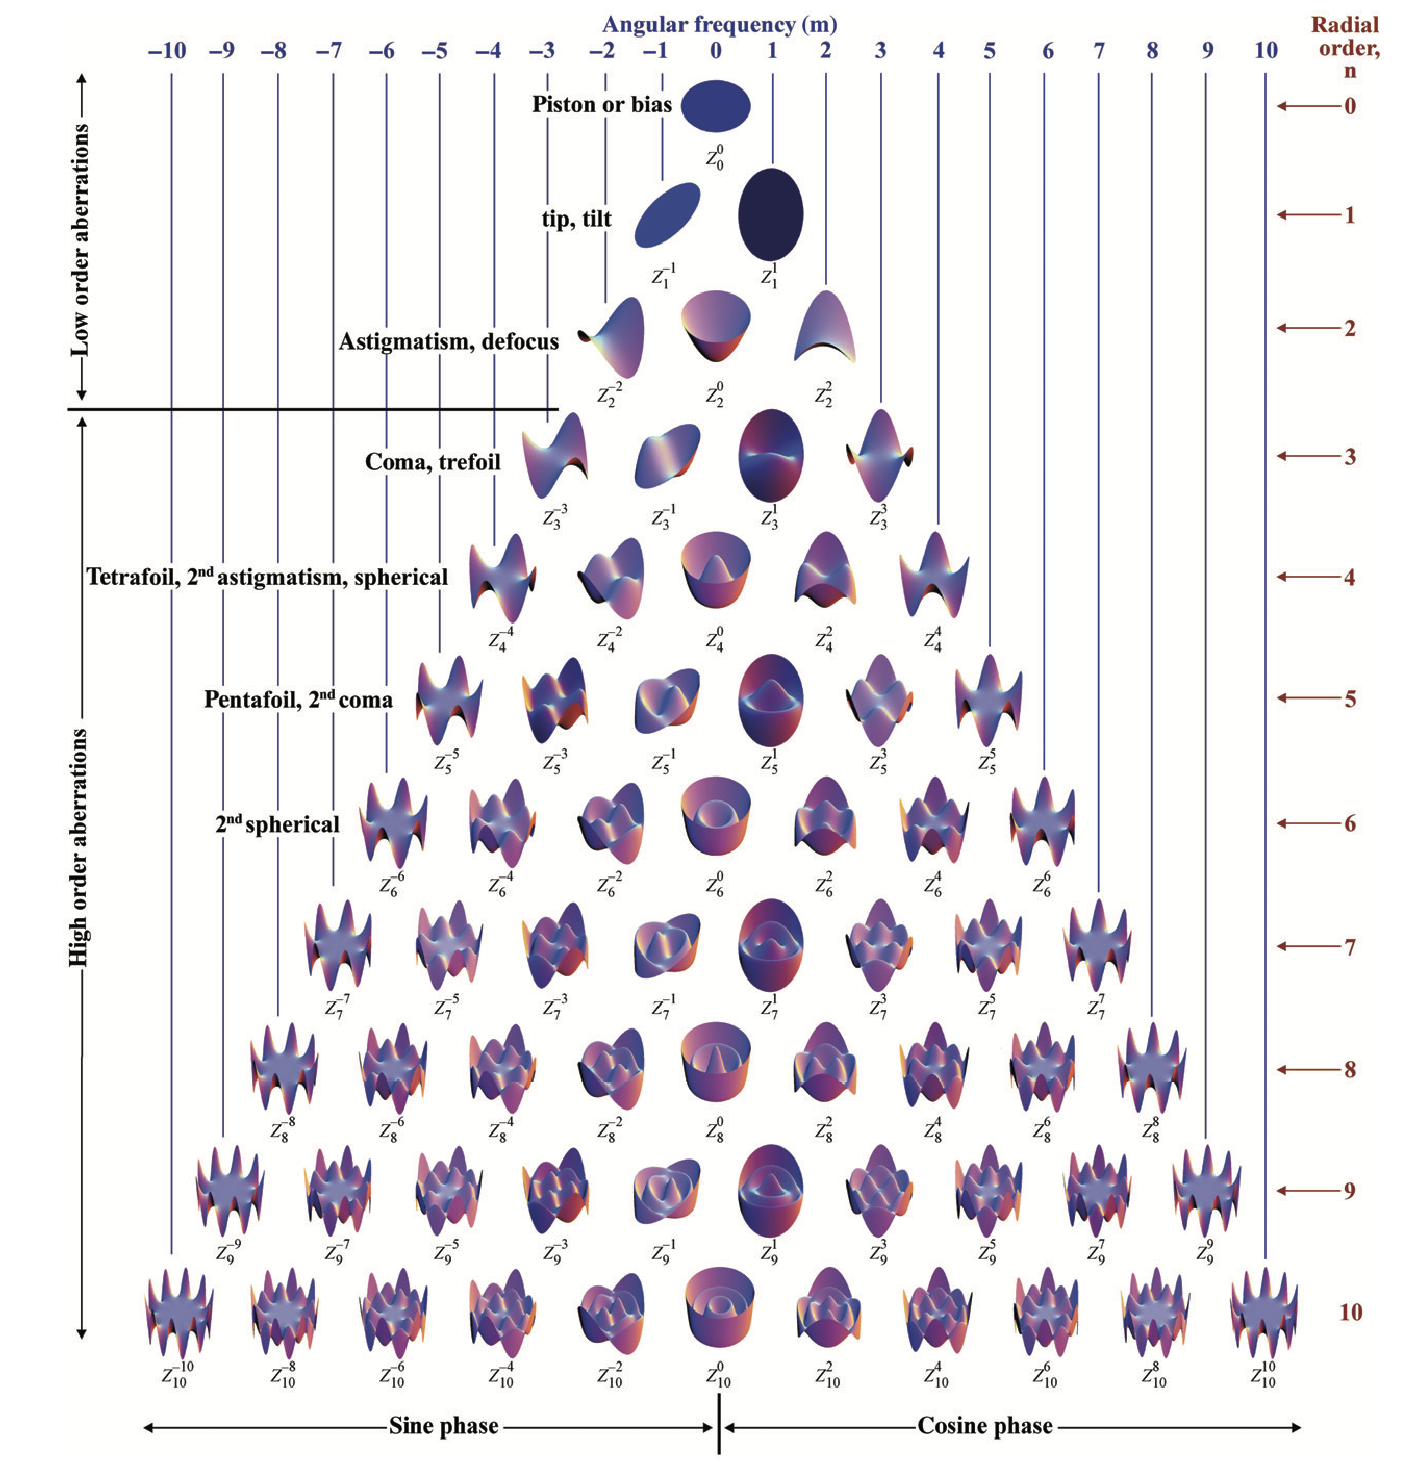
\includegraphics[width=0.7\textwidth]{fig/Zernike.png}
        \caption{Zernike多项式\cite{lakshminarayananZernikePolynomialsGuide2011}}
        \label{zenike}
    \end{figure}
    由于其在单位圆上正交，增加项数不会影响已有项的拟合。Zernike多项式能够与赛德尔像差(Seidel Aberrations)理论对应(见图\ref{zenike})，因而常用以描述圆形光阑系统中的变形的波前。
    \par 这样，只要了解了光瞳函数和像差情况，就能够计算出系统的三维点源扩散函数。按上述方法模拟得到几种典型的3D PSF如下所示：

    \begin{figure}[h]
        \centering
        \setlength{\tabcolsep}{2pt} % 控制列间距
        \renewcommand{\arraystretch}{2} % 控制行间距

        \begin{tabular}{c c c c}  
            % 顶部列名
            \multicolumn{1}{c}{} & \textbf{正常} & \textbf{彗差} & \textbf{像散} \\

            % 第一行
            \textbf{XY投影} &  
            \begin{subfigure}{0.3\textwidth}
                \centering
                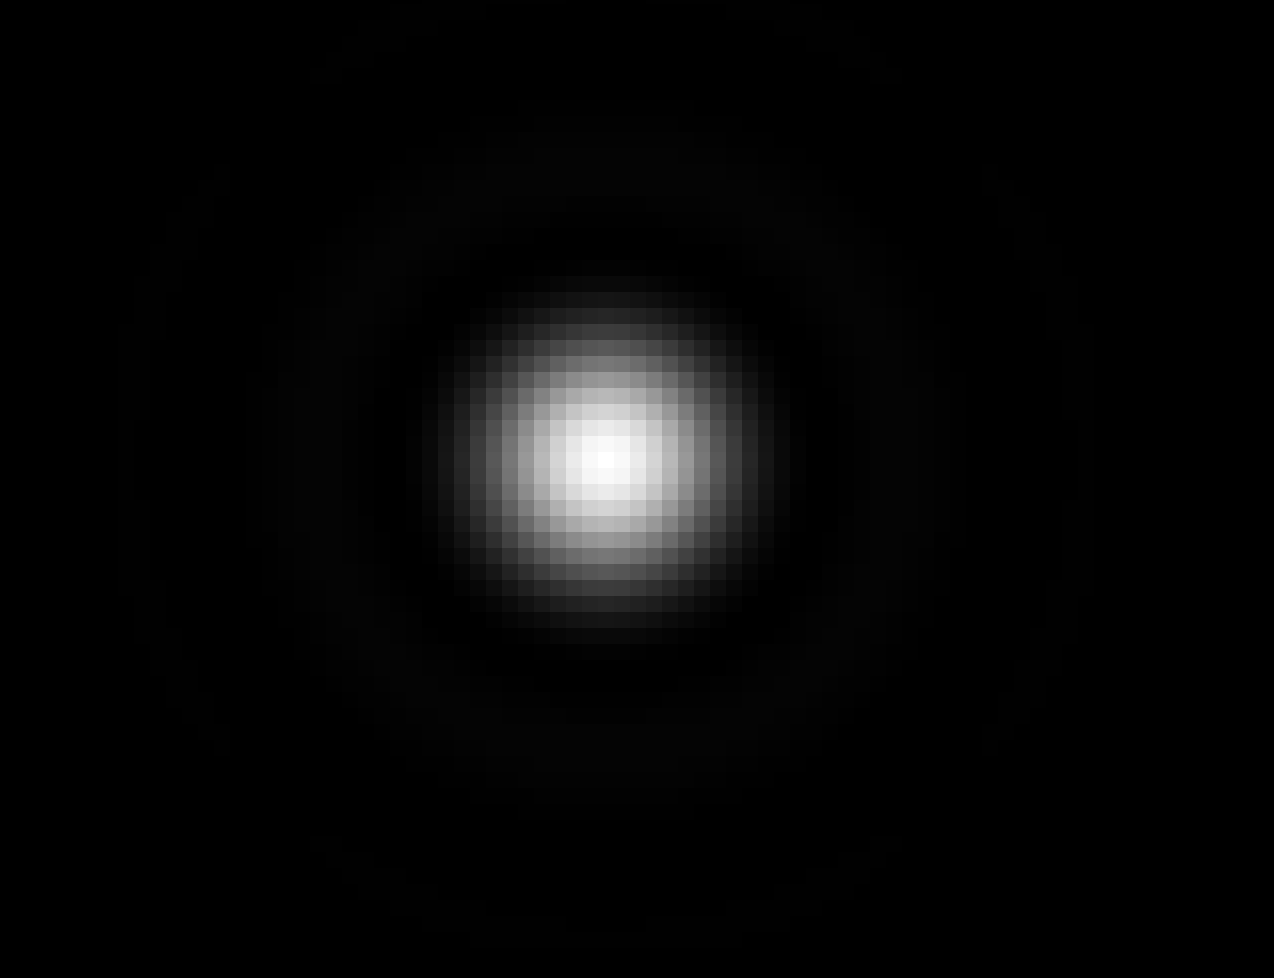
\includegraphics[height=3cm]{fig/normal.png}
            \end{subfigure} &
            \begin{subfigure}{0.3\textwidth}
                \centering
                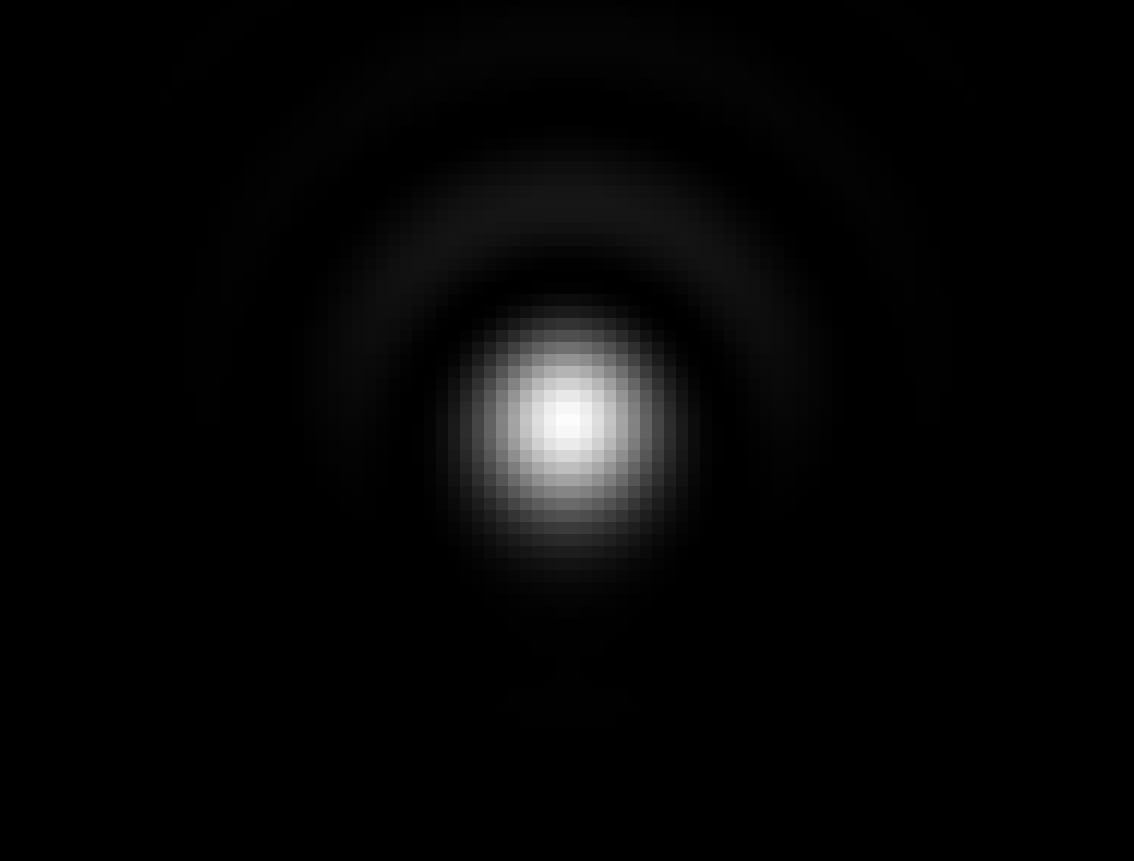
\includegraphics[height=3cm]{fig/coma.png}
            \end{subfigure} &
            \begin{subfigure}{0.3\textwidth}
                \centering
                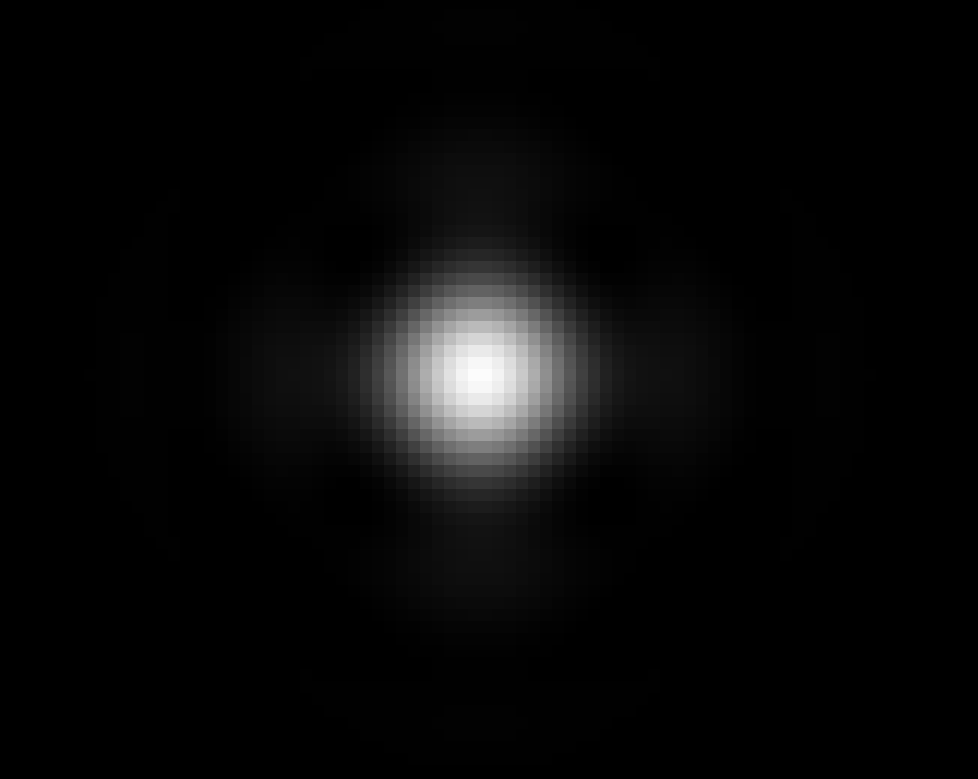
\includegraphics[height=3cm]{fig/astigma.png}
            \end{subfigure} \\

            % 第二行
            \textbf{XZ投影} &  
            \begin{subfigure}{0.3\textwidth}
                \centering
                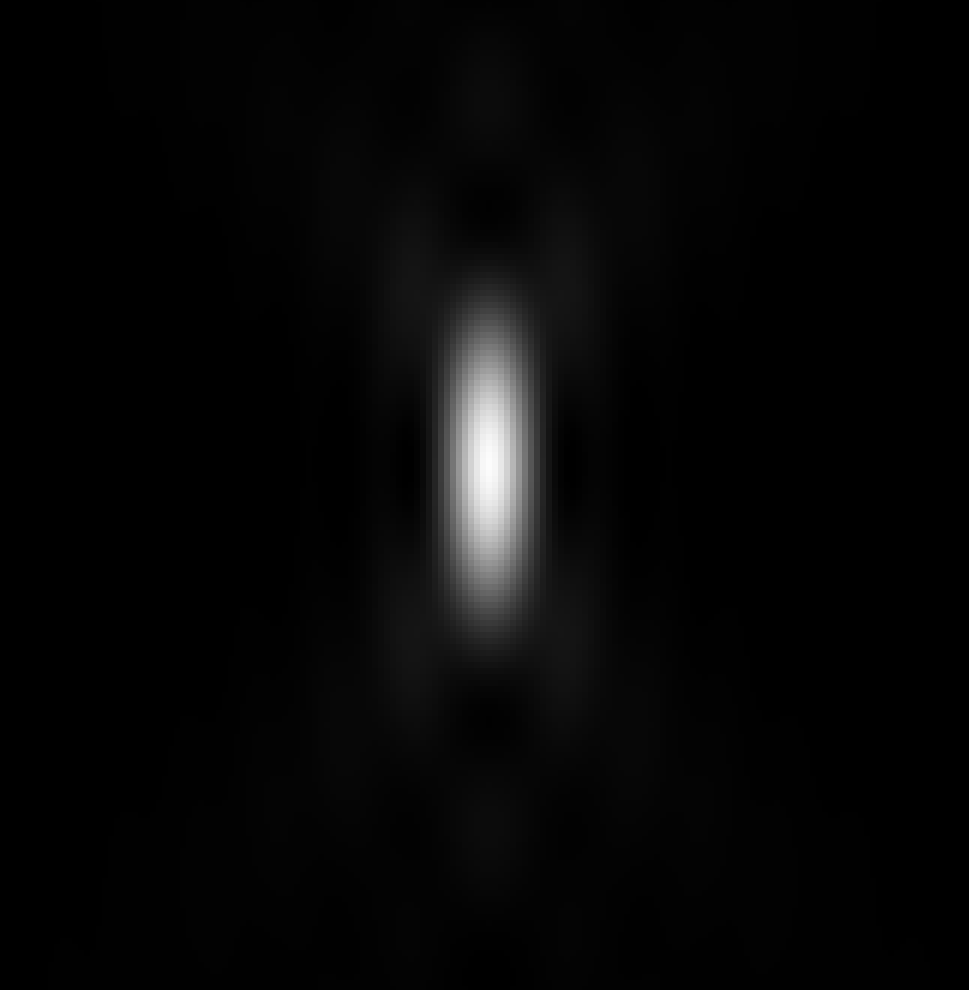
\includegraphics[height=4.2cm]{fig/normal_xz.png}
            \end{subfigure} &
            \begin{subfigure}{0.3\textwidth}
                \centering
                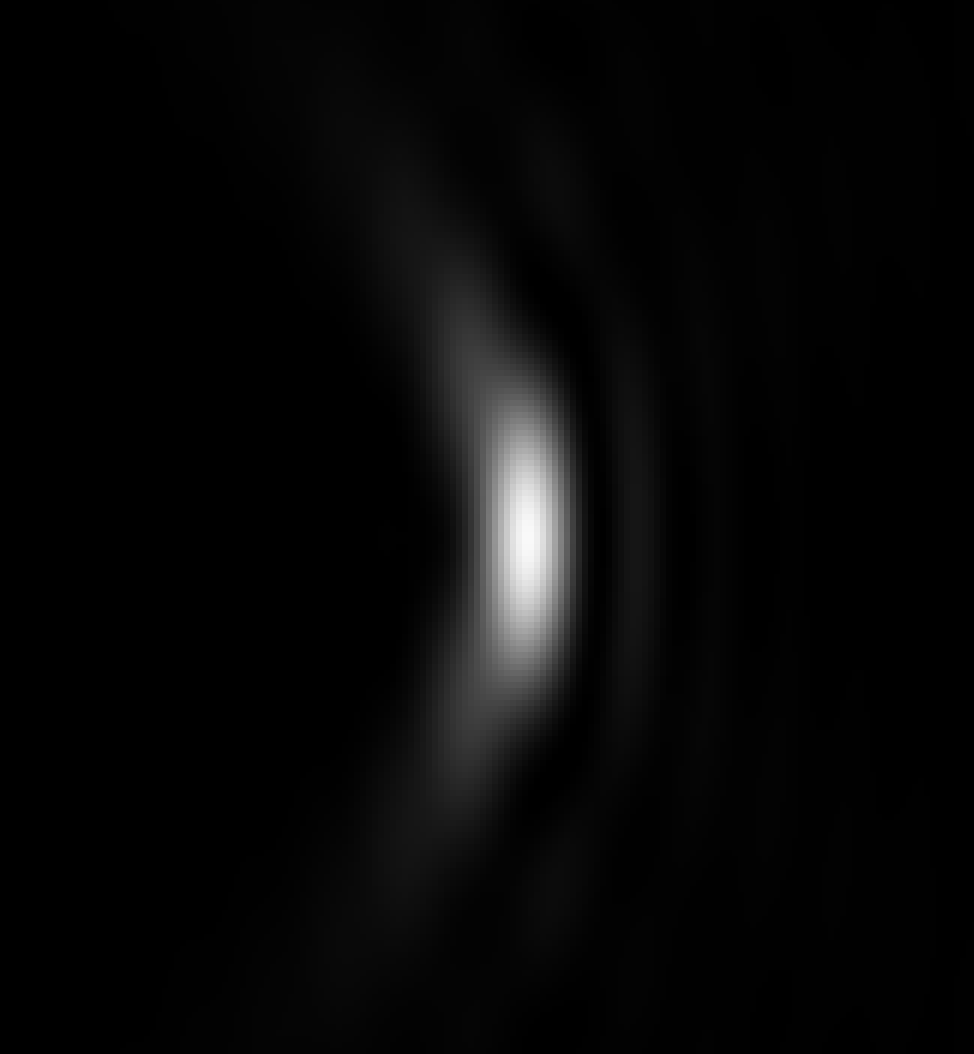
\includegraphics[height=4.2cm]{fig/coma_xz.png}
            \end{subfigure} &
            \begin{subfigure}{0.3\textwidth}
                \centering
                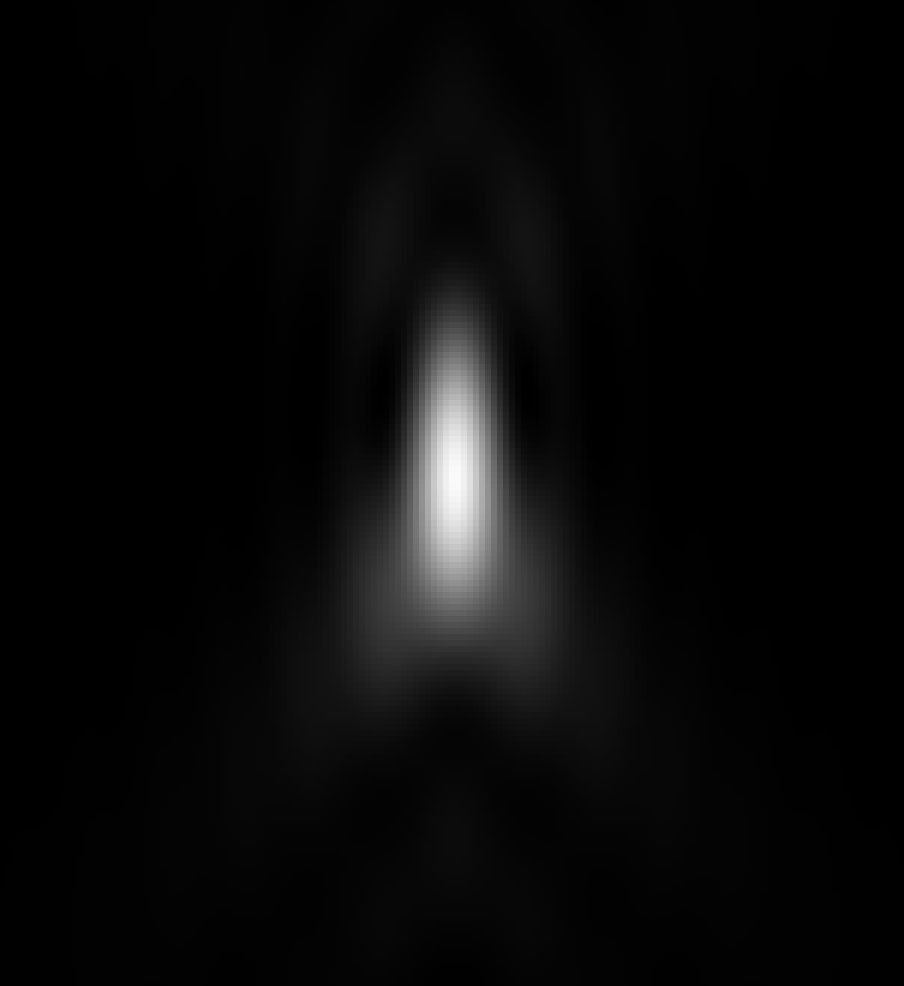
\includegraphics[height=4.2cm]{fig/astigma_xz.png}
            \end{subfigure} \\
        \end{tabular}

        \caption{不同像差的PSF模拟(rms = 0.1 rad)}
        \label{PSF_abe}
    \end{figure}

    \subsection{点源扩散函数工程}
    上述的PSF导出都使用汇聚的傍轴球面波作为传播时的参考，通过Zernike多项式表示与之的相位差，并由于其构成光瞳上的完备基而能够描述大多数像差。而另一方面，复光场本身也可以直接展开到一组傍轴亥姆霍兹方程(paraxial Helmholtz equation)的完备基上，譬如厄米-高斯(hermite-gaussian)函数和拉盖尔-高斯(laguerre-gaussian)函数。后者在截面上具有圆对称的光强分布，并在相位上随z轴螺旋改变。其形式可表示为：
    \begin{equation}
        \begin{aligned}
            U_{l, m}(\rho, \phi, z) & =A_{l, m}\left[\frac{W_{0}}{W(z)}\right]\left(\frac{\rho}{W(z)}\right)^{l} \mathbb{L}_{m}^{l}\left(\frac{2 \rho^{2}}{W^{2}(z)}\right) \exp \left(-\frac{\rho^{2}}{W^{2}(z)}\right) \\
            & \times \exp \left[-j k z-j k \frac{\rho^{2}}{2 R(z)}-j l \phi+j(l+2 m+1) \zeta(z)\right],
            \end{aligned}
    \end{equation}
    \begin{figure}[b]
        \centering
        \begin{subfigure}[b]{0.3\textwidth}
            \centering
            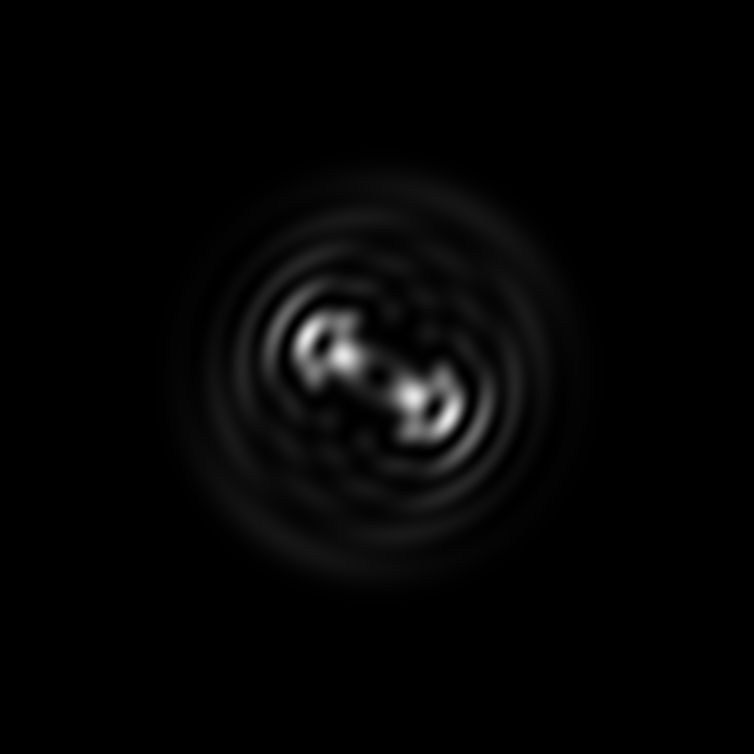
\includegraphics[width=\textwidth]{fig/DH1.png}
            \caption{z=-2um}
            \label{fig:img1}
        \end{subfigure}
        \begin{subfigure}[b]{0.3\textwidth}
            \centering
            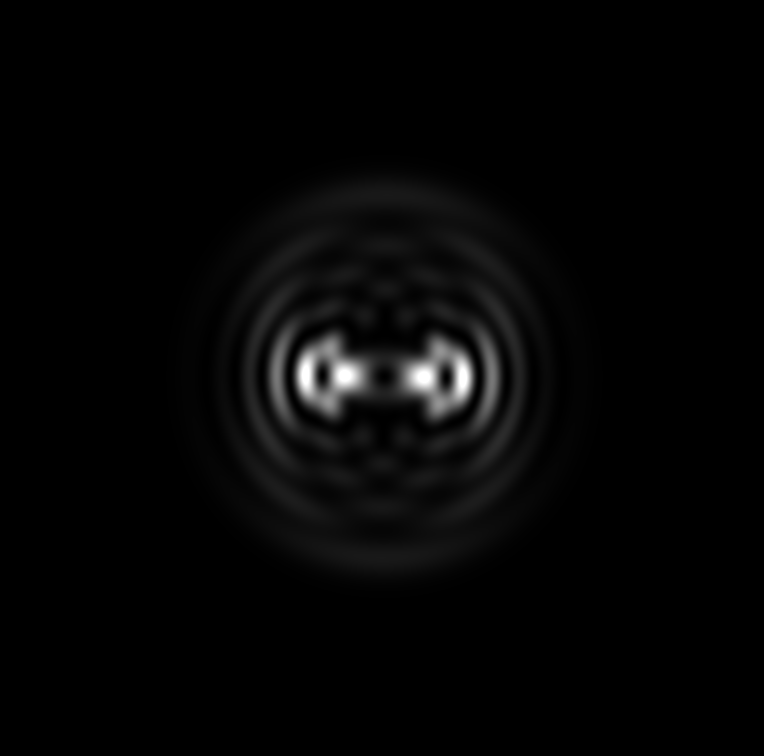
\includegraphics[width=\textwidth]{fig/DH2.png}
            \caption{z=0um}
            \label{fig:img2}
        \end{subfigure}
        \begin{subfigure}[b]{0.3\textwidth}
            \centering
            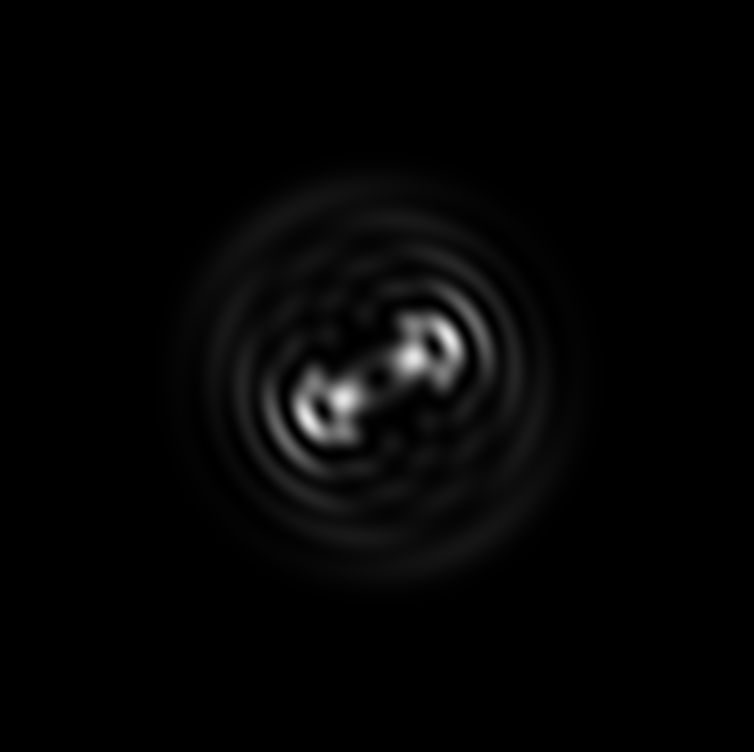
\includegraphics[width=\textwidth]{fig/DH3.png}
            \caption{z=2um}
            \label{fig:img3}
        \end{subfigure}
        \caption{双螺旋PSF}
        \label{fig:DH}
    \end{figure}
    其中每一个模态由角序数和径向序数$(l,m)$决定，$\mathbb{L}_{m}^{l}$为连带拉盖尔多项式。这些集函数能够通过相同能量的线性组合产生具有自相似性(generalized self-imaging)，譬如不断旋转的PSF，见文献\cite{piestunPropagationinvariantWaveFields2000}。按照(1,1)(3,2)(5,3)(7,4)(9,5)序数的等强组合作为掩膜可以计算得到如图\ref{fig:DH}的3D PSF。注意光强分布随着z轴保持形状并绕轴旋转，这可以作为z轴定位的指示。不过，如绪论中所述，经过改造的PSF体积变大，相对而言更不利于密集的定位和算法拟合。

    
    \section{离散化的处理}
    由于图像处理器是离散化的点阵，最终获得的图像相当于以像素尺寸$(\Delta x,\Delta y)$为间隔、以处理器总尺寸$(L_x, L_y)$为周期的二维离散信号。根据采样和周期性的傅立叶变换性质，其离散傅里叶变换后的频谱具有采样频率：
    \begin{equation}
        \Delta f_x=\frac{1}{L_x},\Delta f_y=\frac{1}{L_y}
    \end{equation}
    比方说X方向上10微米*128像素的传感器，其离散傅里叶变换后的频率坐标间隔是：
    \begin{equation}
        \Delta f_x=\frac{1}{10\mu m*128}=781.25 \ m^{-1}
    \end{equation}
    \par 在计算机上所有数据都是离散化的，因而只需记录并储存每个离散值坐标对应的实际物理量就可以准确进行换算。在程序中，首先根据NA和$\lambda$等参数构建频域中光瞳函数的网格，然后将生成的像差和离焦像差整合进其中，利用快速傅里叶变换（FFT）即可快速计算三维点源扩散函数，其同随机生成的点源卷积即可得到三维的模糊(blurred)图像k。在附录代码中使用了上采样网格来进行更高精度的PSF计算，在模拟实际数据时通过下采样匹配使用的CCD即可。

    \section{噪声的添加和信息矩阵}
    \subsection{噪声模拟}
    实际成像中，由于如式(\ref{emit})所表示的光子发射过程的随机性，每个像素上的信号将是以其大小为均值的泊松分布(poisson distribution)：
    \begin{equation}
        S_{\theta,k}\sim Poisson(\gamma At\int_kf_{\theta}(\textbf{r})d\textbf{r})=Poisson(s_{\theta,k}\ t)
    \end{equation}
    其中系数$\gamma At$代表传感器接受到来自一个点源的信号的总量，$k$代表像素的编号，$f_{\theta}(\textbf{r})$是上文所述归一化PSF，在第k个像素对其进行积分得到分布概率。在模拟中可通过设置点源的平均发射数来代替。除此外，还需添加远处背景造成的随机柏松噪声和传感器造成的白噪声：
    \begin{equation}
        B_{\theta,k} \sim Poisson(\beta_{\theta,k}\ t) , \ W_{k} \sim Gaussian(\eta,\sigma_k)
    \end{equation}

    \begin{figure}[h]
        \centering
        \begin{subfigure}[b]{0.4\textwidth}
            \centering
            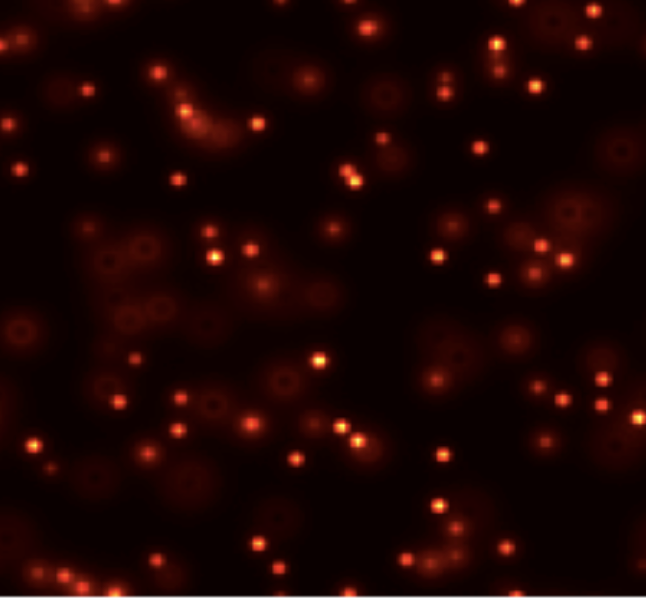
\includegraphics[width=\textwidth]{fig/unblured.png}
            \caption{理想点源}
        \end{subfigure}
        \begin{subfigure}[b]{0.4\textwidth}
            \centering
            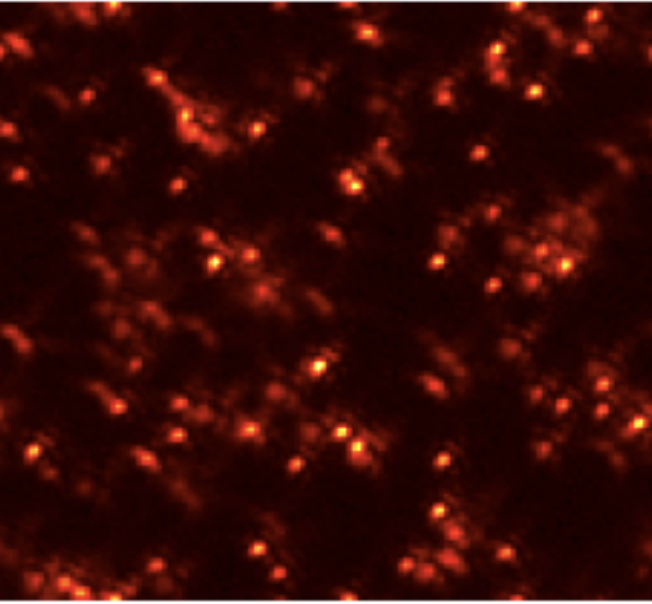
\includegraphics[width=\textwidth]{fig/blured.png}
            \caption{含像差和噪声的点源}
        \end{subfigure}
        \caption{添加噪声和像差后的模拟图像}
        \label{Noise}
    \end{figure}
    \par 注意$\theta$可能包含坐标、亮度、背景等多个估计参数。将这三项相加即可模拟点源的成像信号。这一般可用以对CMOS和CCD类的传感器噪声进行模拟。其他种类的图像传感器噪声模型参见文献\cite{chaoFisherInformationTheory2016}。按上述模型得到的模拟数据集如图\ref{Noise}所示。

    

    \subsection{定位精度下限分析}
    注意到单分子成像的目标是定位单分子坐标，而后者可看作是模型的待定参数。根据统计估计理论，我们可以计算任意无偏估计器(unbiased estimator)的方差下限，即Cramér–Rao下界。其可由费歇尔信息(Fisher Information)矩阵的逆求出：
    \begin{equation}
        \textup{Var}\ \hat{\theta_i} \geq \textbf{I}^{-1}(\theta)_{ii}
    \end{equation}
    其中费歇尔矩阵定义为：
    \begin{equation}
        \textbf{I}(\theta)=\mathbb{E}\ (\frac{\partial \ln \mathbb{P}\{X=x|\theta\}}{\partial \theta})^{T}(\frac{\partial \ln \mathbb{P}\{X=x|\theta\}}{\partial \theta})
    \end{equation}
    \par 其中求偏导的项称为对数似然函数，描述了在某模型参数下给定实验结果的可能性。信息矩阵定义为对数似然函数对参数的偏导数的平方的期望，直观含义为平均而言的随机数据对模型参数的敏感性——愈不敏感的数据愈平凡，亦即我们能期望从中获得关于参数的信息愈少。因而我们能建立其和估计精度的关联。
    \par 根据上一节定义的模型，可以导出信息矩阵：
    \begin{equation}
        \begin{aligned}\mathbf{I}(\theta)= & \sum_{k=1}^{K}\left(\frac{\partial \nu_{\theta, k}}{\partial \theta}\right)^{T}\left(\frac{\partial \nu_{\theta, k}}{\partial \theta}\right) \\& \times\left(\int_{-\infty}^{\infty} \frac{\left(\frac{e^{-v_{\theta, k}}}{\sqrt{2 \pi} \sigma_{k}} \sum_{l=1}^{\infty} \frac{\nu_{\theta, k}^{l-1}}{(l-1)!} e^{\frac{-\left(z-l-\eta_{k}\right)^{2}}{2 \sigma_{k}^{2}}}\right)^{2}}{p_{\theta, k}(z)} \mathrm{d} z-1\right),\end{aligned}
    \end{equation}
    其中$\nu_{\theta, k}=s_{\theta,k}+\beta_{\theta,k}$,详细的导出参见附录。
    由于如是计算的方差表示能够达到最好的估计精度，所以对每一组模拟参数，都可以计算其定位精度下限以作为待评估模型“改进空间”的参考。而方差低于该下限的估计器很可能出现了过拟合的现象，需要仔细检查其模型的合理性。
    
    \chapter{编解码器神经网络的架构和训练}
    通过第二章中的方法，我生成了不同点源密度和信噪比、含有13阶次随机像差的模拟数据集，其中zernike系数的1，2，4阶不算在内（排除x，y倾斜和离焦像差）。现考虑从含像差、噪声的图像到不含噪声的图像的映射，即输入和输出为相同尺寸的二维图像。换言之，此时模型需要去除1.噪声 2.像差。通过使用计算出的不含像差和噪声的理想图像作为ground truth，我们期望模型能够1.捕获到细微的衍射图样 2.自行整合此类信息以判断整张图像的像差 3.还原出原本的图像。卷积神经网络对图像中的空间关系敏感，因而成为该模型的首选结构。
    \section{网络结构和细节}
    因为输入和输出皆为图像，编码-解码结构符合上述对模型的要求。在每一次编码时，选用多个一定尺寸的卷积核，通过设置步长(stride)以在缩小图像尺寸的同时拓展通道数(channel)，最终将图像编码为一串“特征”；而解码部分则与之相反，负责将”特征“还原为图像。本文使用的架构每次将原图尺寸压缩一半，在编码阶段经过4层、解码阶段为3层，其原理见简化图\ref{mynet}。
    \begin{figure}[h] 
        \centering
        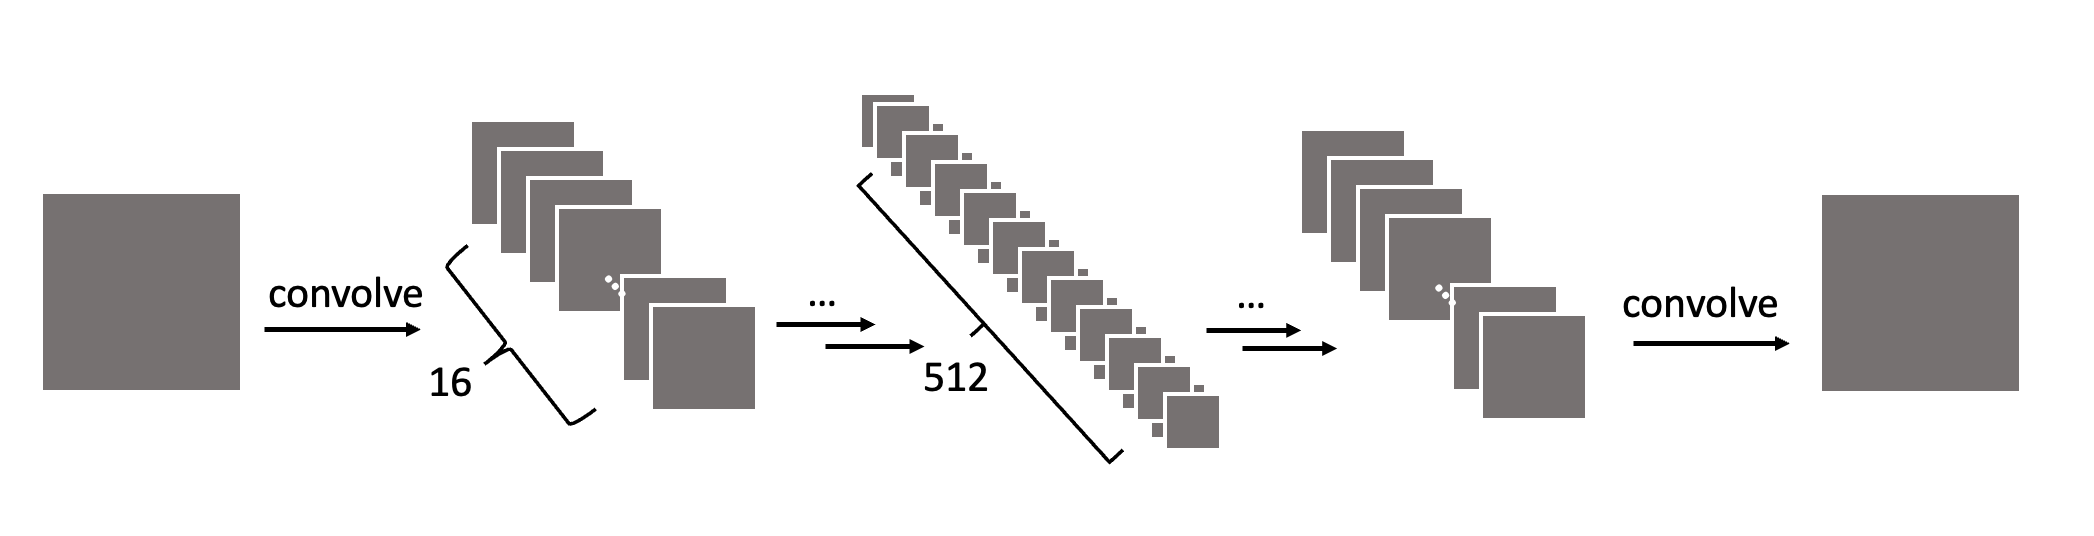
\includegraphics[width=0.7\textwidth]{fig/mynet.png}
        \caption{DeAbe网络结构示意}
        \label{mynet}
    \end{figure}
    \par 作为区别于线性模型的关键，每一层进行卷积操作后，还需要施加一个非线性函数。本文中选取广泛使用的ReLu函数，以加速计算和缓解梯度消失(Vanishing gradient)等问题。此外，为了防止层数过多导致的不稳定的问题，在每次施加ReLu函数前额外使用BatchNorm2d进行正则化，即根据其标准差调整其参数的分布范围，否则如此深度的网络具有将图像全部归零的倾向。网络使用kaiming初始化以增加训练时候的稳定性(尽量保持隐藏变量/梯度的方差不变)。

    \section{损失函数和训练方法}
    由于单分子点源本身的稀疏性，本文采用了混合了L1和L2范数的损失函数(loss function):
    \begin{equation}
        Loss(\hat{y},y)=\alpha (\sum_i(\hat{y}_i-y_i)^2)+(1-\alpha)(\sum_i|\hat{y}_i-y_i|)
    \end{equation}
    其中L1范数对小量施加更多的惩罚，因而在无源处的惩罚比L2范数更有力，有助于形成稀疏的输出。按常规做法，选择torch.optim库中的Adam优化器。数据集在转化为torch张量后随机按8:2的比例分成训练集(training set)和测试集(test set)，其中测试集直最后都不参与训练过程。训练集按小批次(mini batch)对模型进行优化，批次数量的具体选择可根据图形处理器性能决定。由于损失函数较难直观判断图像相似度信息，选用结构相似性指数(ssim)对数据进行可视化的跟踪。所有计算在apple m3 mps上进行；当使用6000张128*128像素图像作为数据集（点源密度跨越一个数量级）、批次大小设置为64时，100次迭代优化的结果如图\ref{train}，用时90min。
    \begin{figure}[h] 
        \centering
        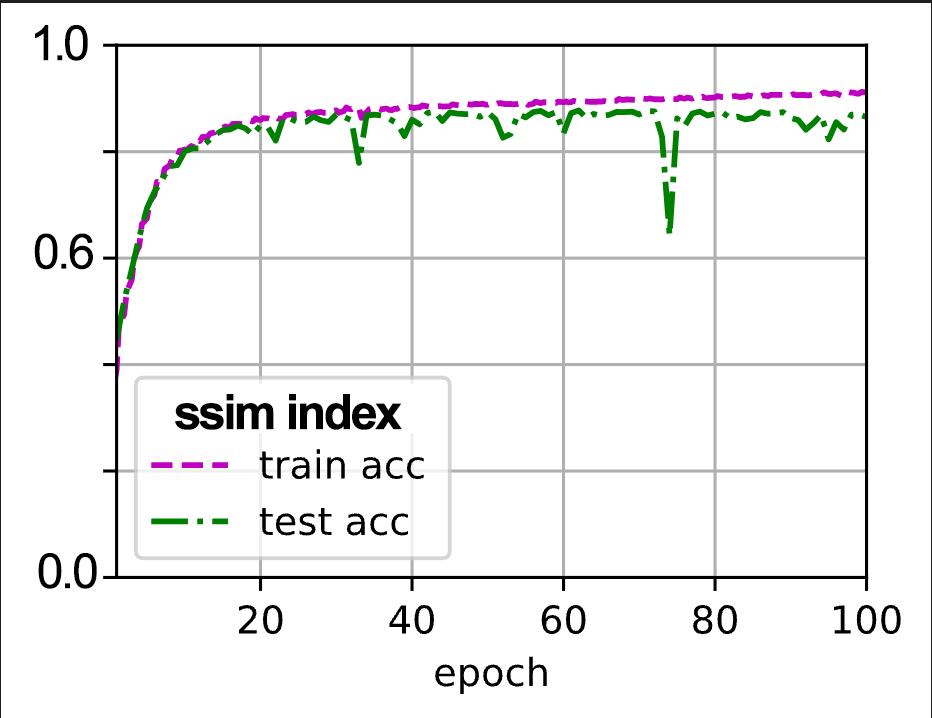
\includegraphics[width=0.7\textwidth]{fig/train.png}
        \caption{ssim随训练轮次的变化}
        \label{train}
    \end{figure}
    \par 注意到约50轮次后测试集上的相似度就不再显著变化，而是在0.85附近波动，而训练集上的相似度仍然在提高。这说明此时模型已经倾向于对数据过拟合了。一般来说，增加数据量或同时增加网络的复杂度能够提高泛化能力，然而这也会显著增加训练时间。下面我们考察该6000张图训练得到的模型效果。
    \begin{figure}[h] 
        \centering
        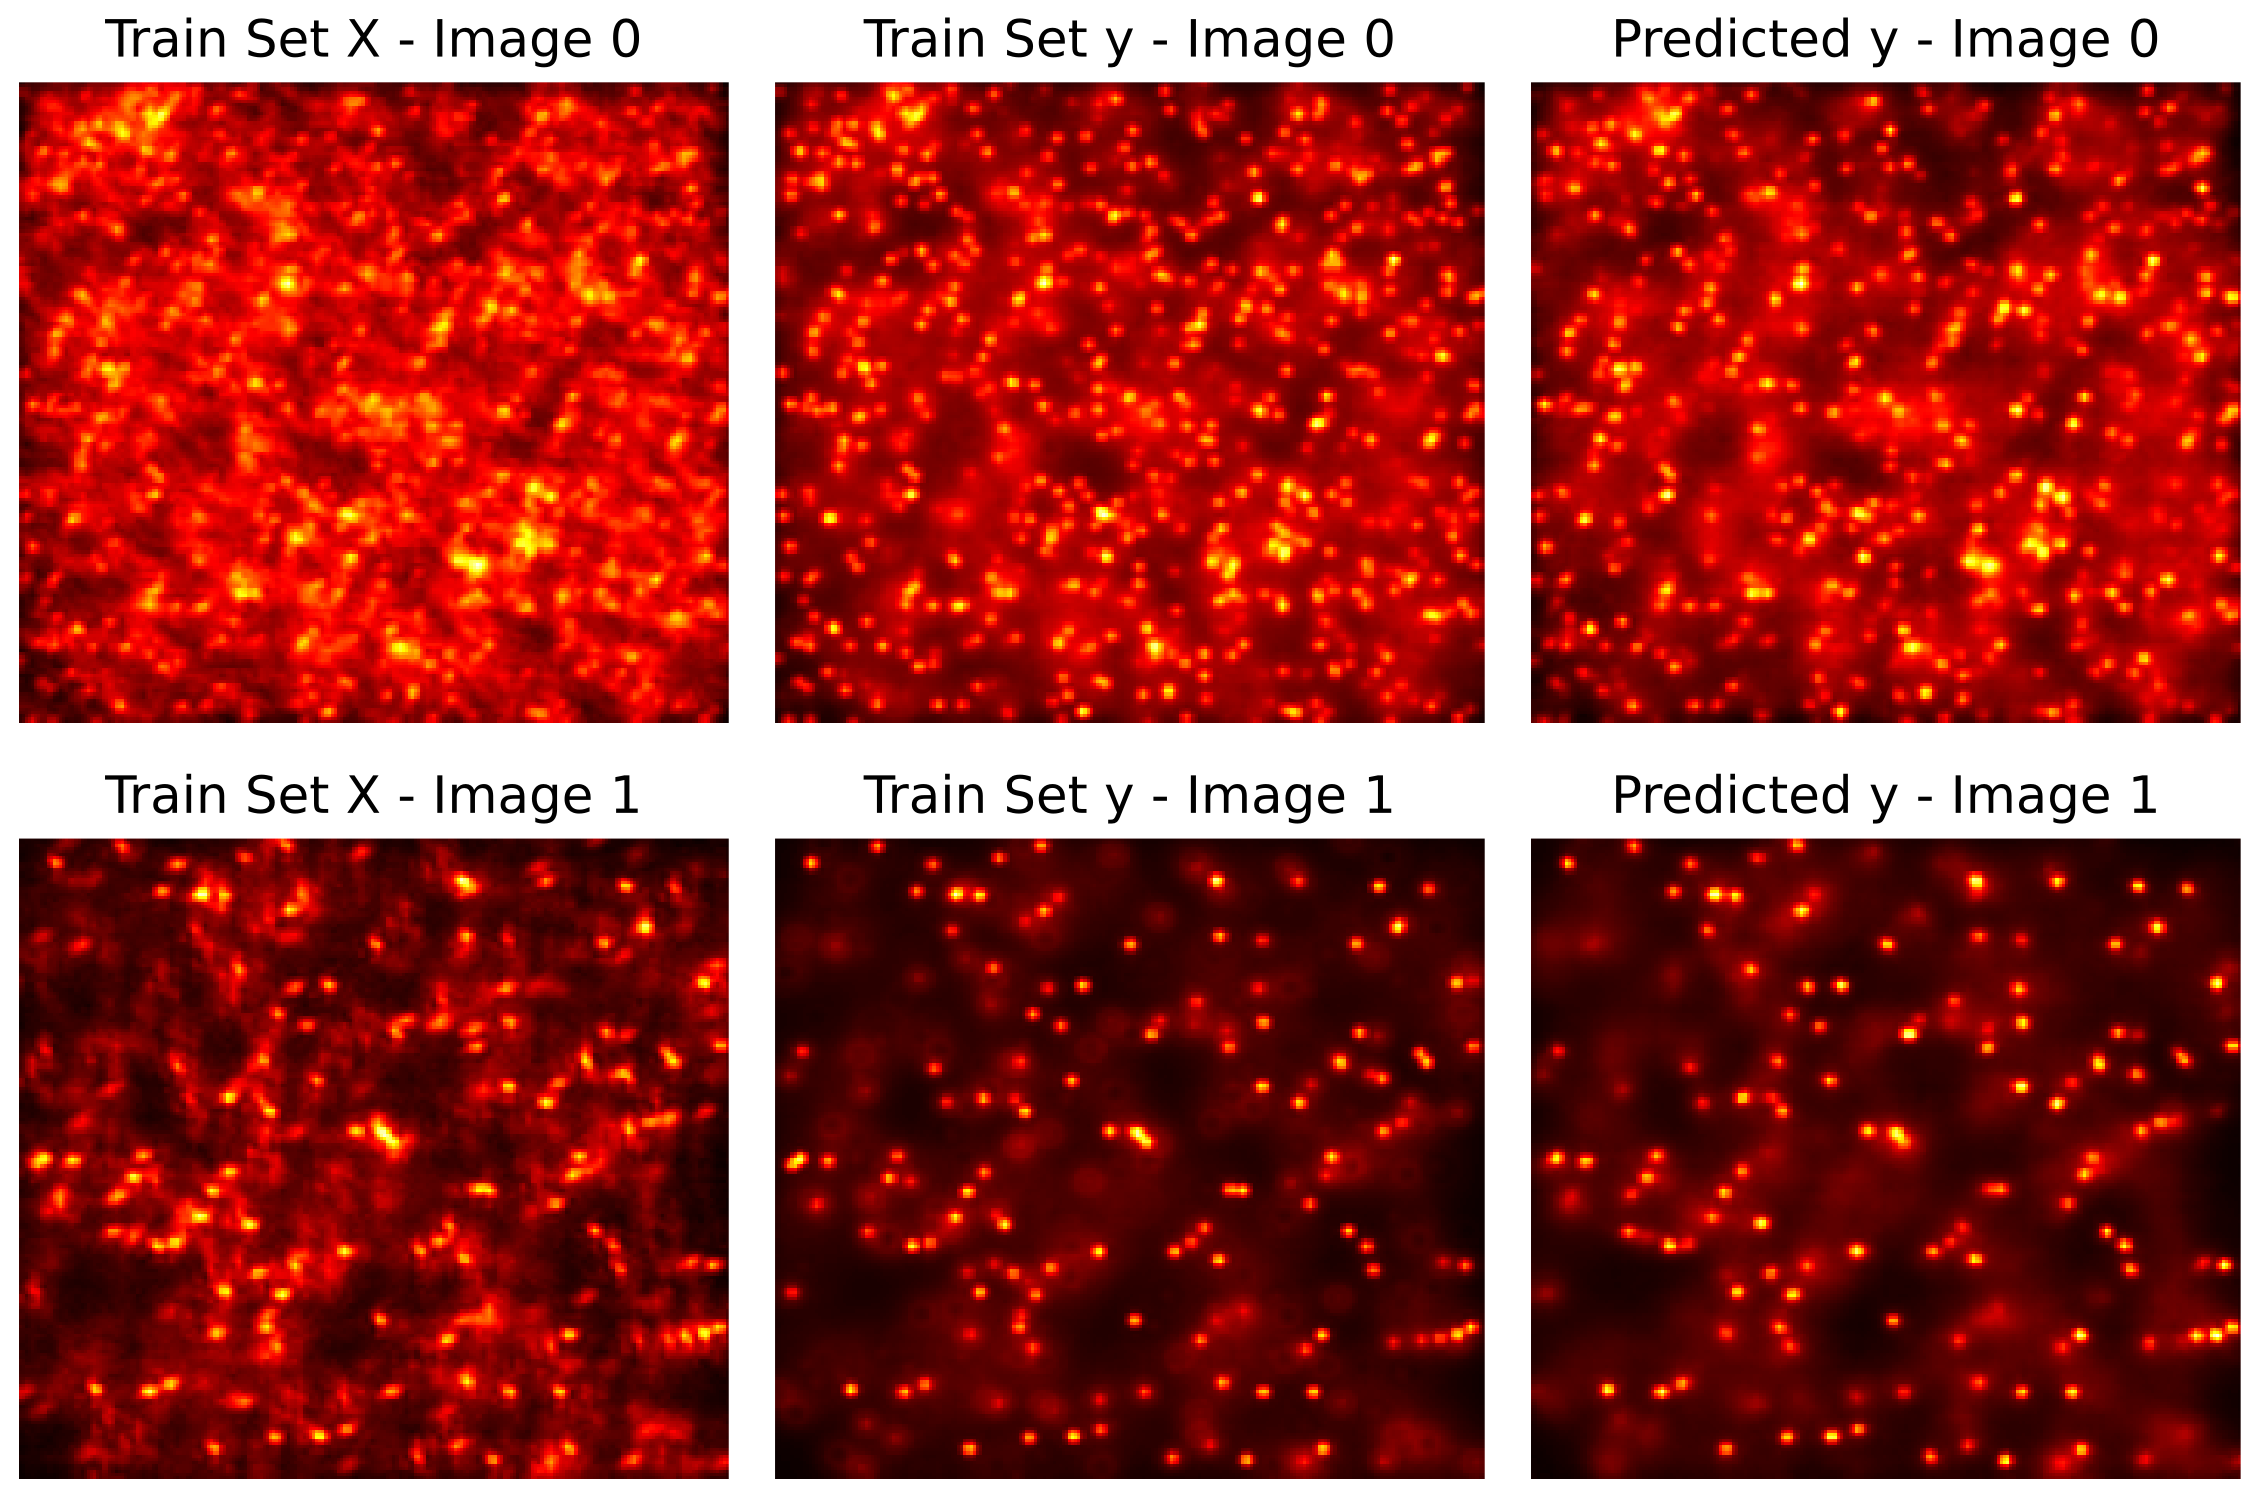
\includegraphics[width=0.7\textwidth]{fig/exp.png}
        \caption{模型对高密度、低密度的含像差图片的恢复能力示意}
        \label{exp}
    \end{figure}

    \section{模型效果比对}
    
    从测试集中随机抽取高密度和低密度点源的两张图片，见图\ref{exp}。中间为ground truth，即不含像差和噪声的理想图像。
    可见模型对其具有矫正能力，其中高密度场景下的恢复能力较为有趣，由于训练集中的点源是随机生成的，理论上亦可用于有规律的点源，如标记在生物结构上的点源。这说明该网络可能亦具有矫正普通非超分辨图像的像差能力，从而恢复到衍射置限的水准。另外，由于训练集数据包含了失焦信息，而非只还原出xy平面的信息，还原的图像在离焦区域能够显示出弥散圆，这对准确还原原始信息是有益的。
    \begin{figure}[h] 
        \centering
        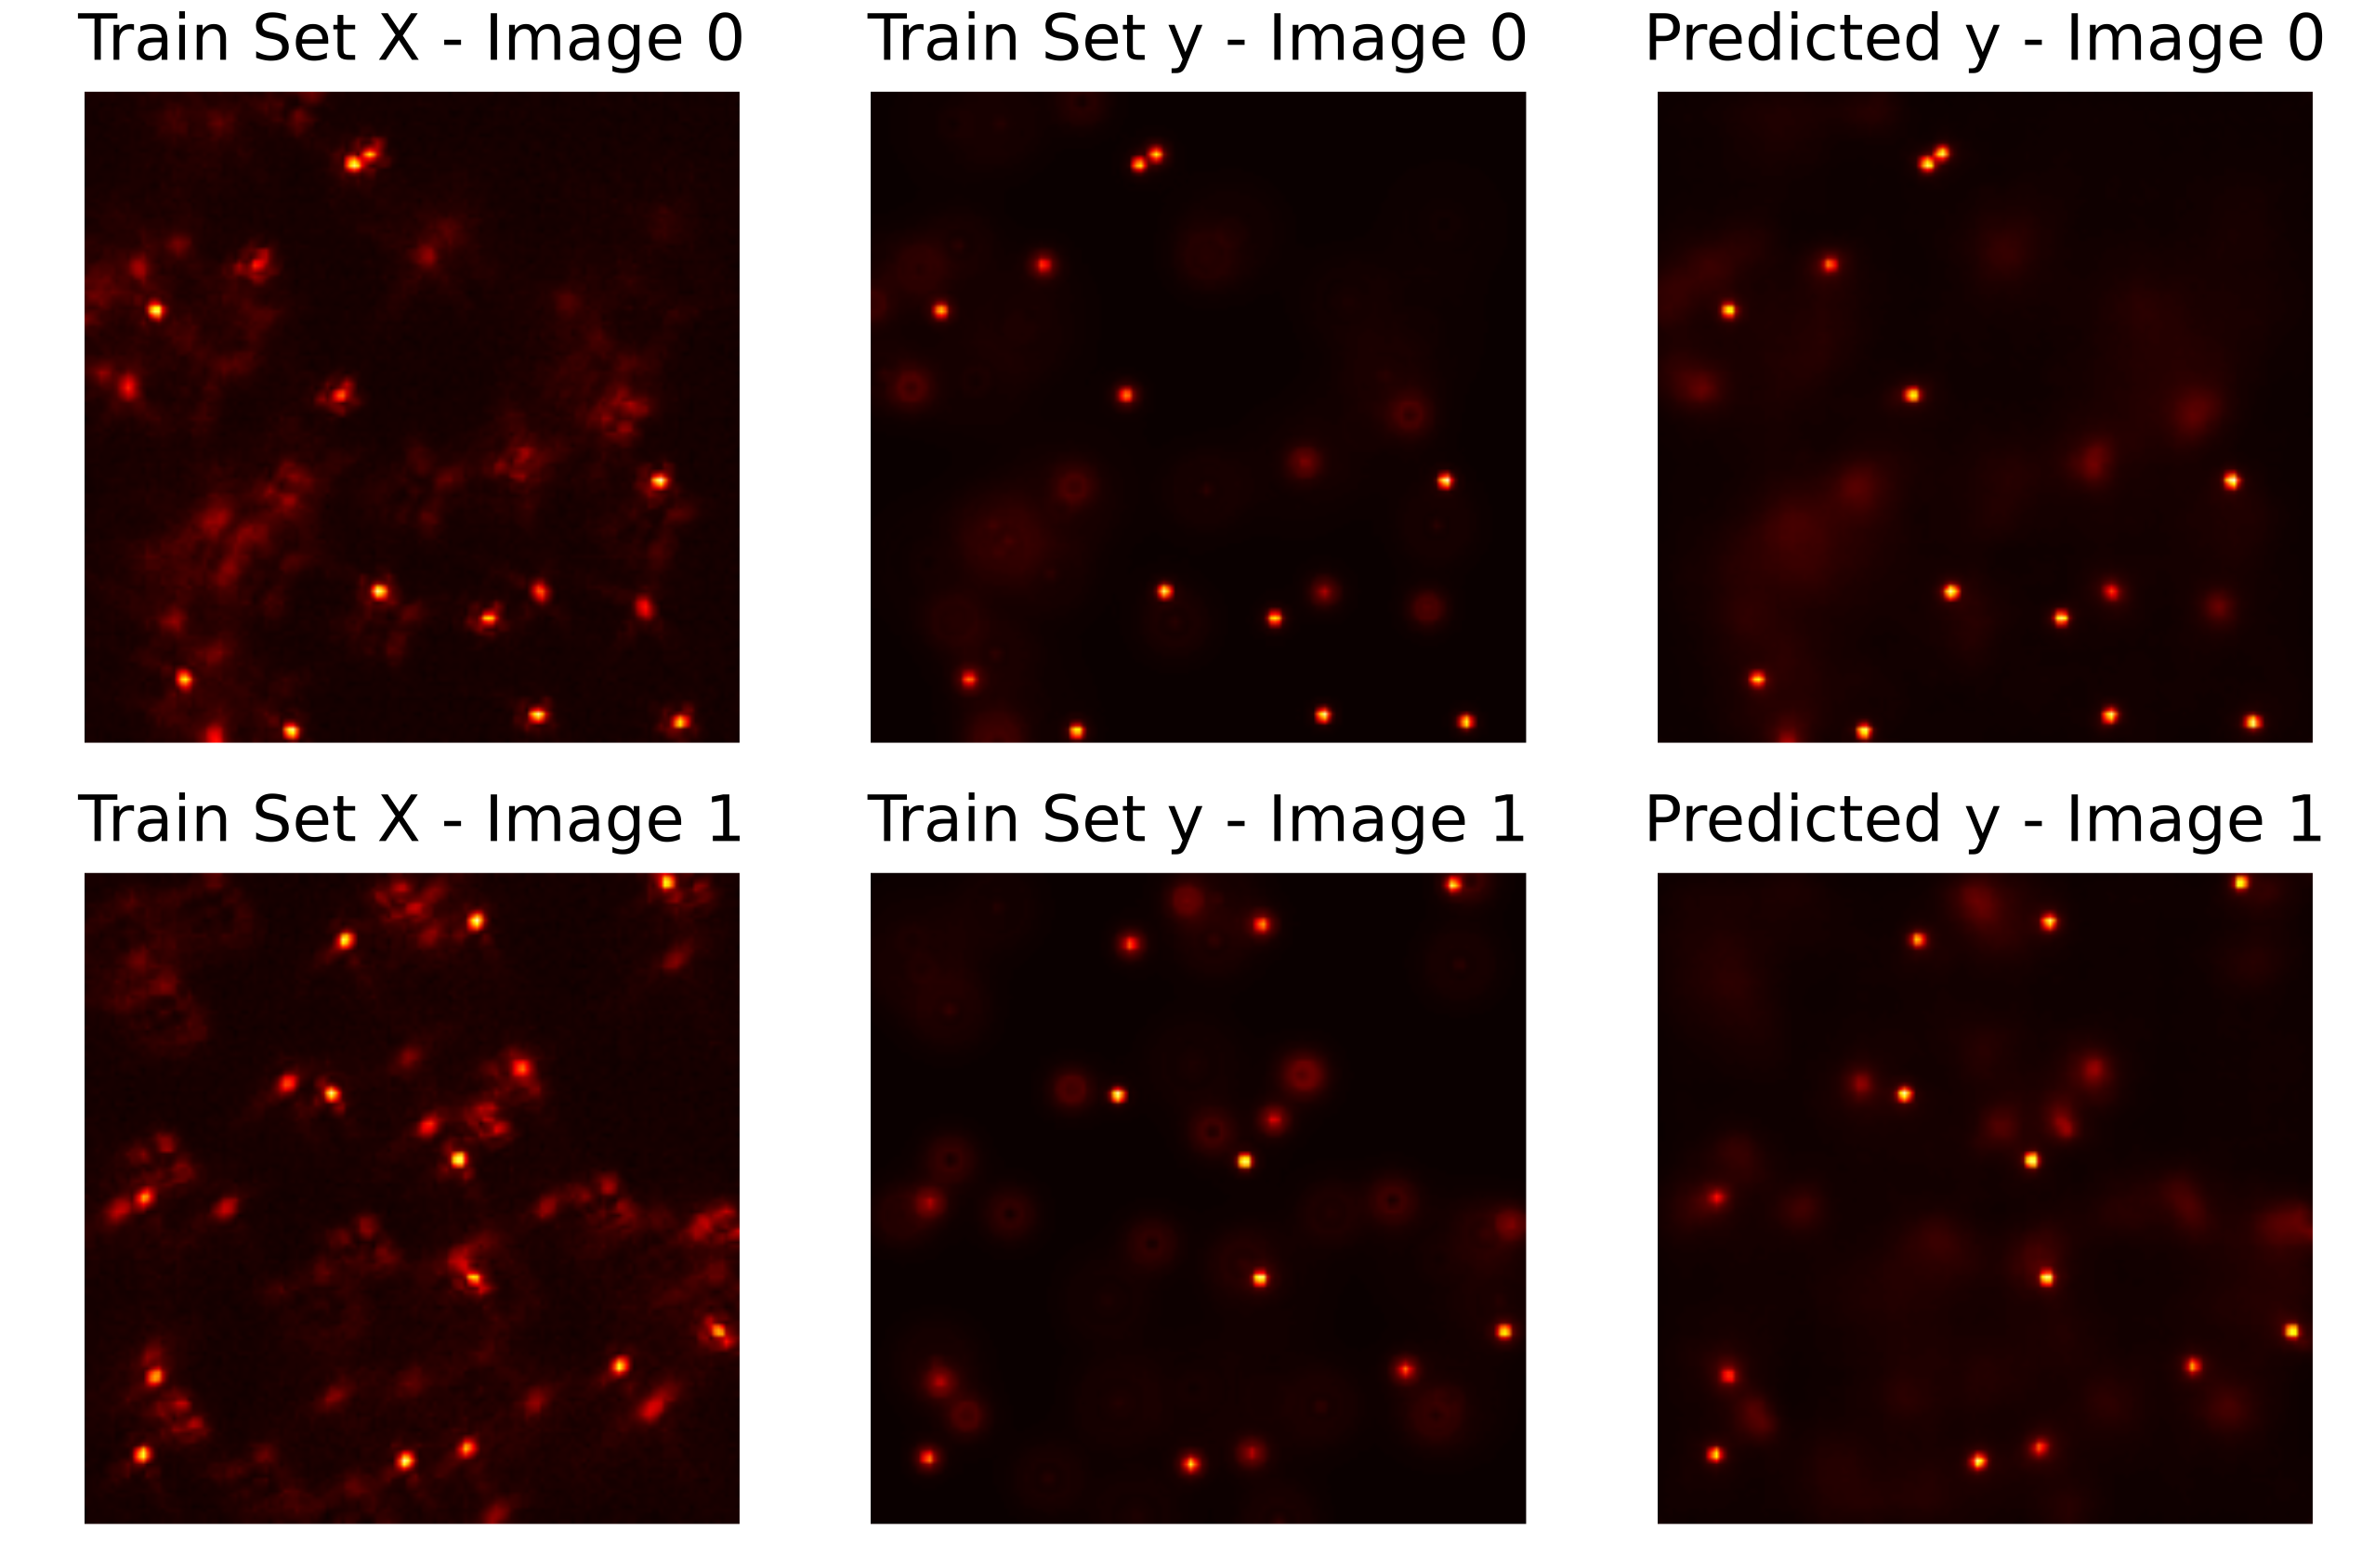
\includegraphics[width=0.7\textwidth]{fig/exp_LOW.png}
        \caption{模型对新生成的低密度的含像差图片的恢复能力示意}
        \label{exp_LOW}
    \end{figure}
    \par 使用另外生成的更低密度的数据，可见模型对此前未“见过”的数据亦具有一定的矫正能力，说明其具有潜在的泛化能力，见图\ref{exp_LOW}。换言之，该模型对点源密度具有一定的鲁棒性。
    \par 为了量化模型的矫正能力，将原始图像和输出的图像使用ThunderSTORM软件包对上述低密度分子进行定位；使用低密度数据可以排除定位重叠的复杂性。背景按模拟时的预设，检测方法为局部极值(Local maximum)，定位方法为加权最小二乘法(Weighted Least squares)。软件包输出的定位导出为csv文件，将之与模拟时使用的准确坐标进行比对，保留其周围6个亚像素，即半径130nm内的定位。为确保严重离焦的点源不影响定位精度的计算，将定位点源限制在20个亚像素、即焦面上下433nm的空间内。
    \begin{table}[!htbp]
        \caption{去像差网络对定位精度的提升} 
        \centering
        \begin{tabular}{c c c}
            \toprule[2pt]
                 & 识别率(\%) & 准确度(nm) \\
            \midrule 
            原始图像 & 95 & 42.7 \\
            去像差后 & 99 & 28.2 \\
            \bottomrule [2pt]
        \end{tabular}
        \label{compare2}
    \end{table}
    \par 测试共使用了180帧、共2049个点源坐标。作为参考，同时对不含像差的图像(即训练时使用的ground truth)进行定位，则得到所有定位中，经过去像差的图像识别出99\%的点源，而未经处理的含噪声图像识别出95\%的点源。对这些点源进行准确度的计算，则经过去像差的图像达到28.2nm，而未经处理的含噪声图像准确度为42.7nm(作为参考，ground truth的图像定位精度为3.9nm，由于像素化误差导致)，见表\ref{Thm}。
    \begin{figure}[h]
        \centering
        \begin{subfigure}[b]{0.3\textwidth}
            \centering
            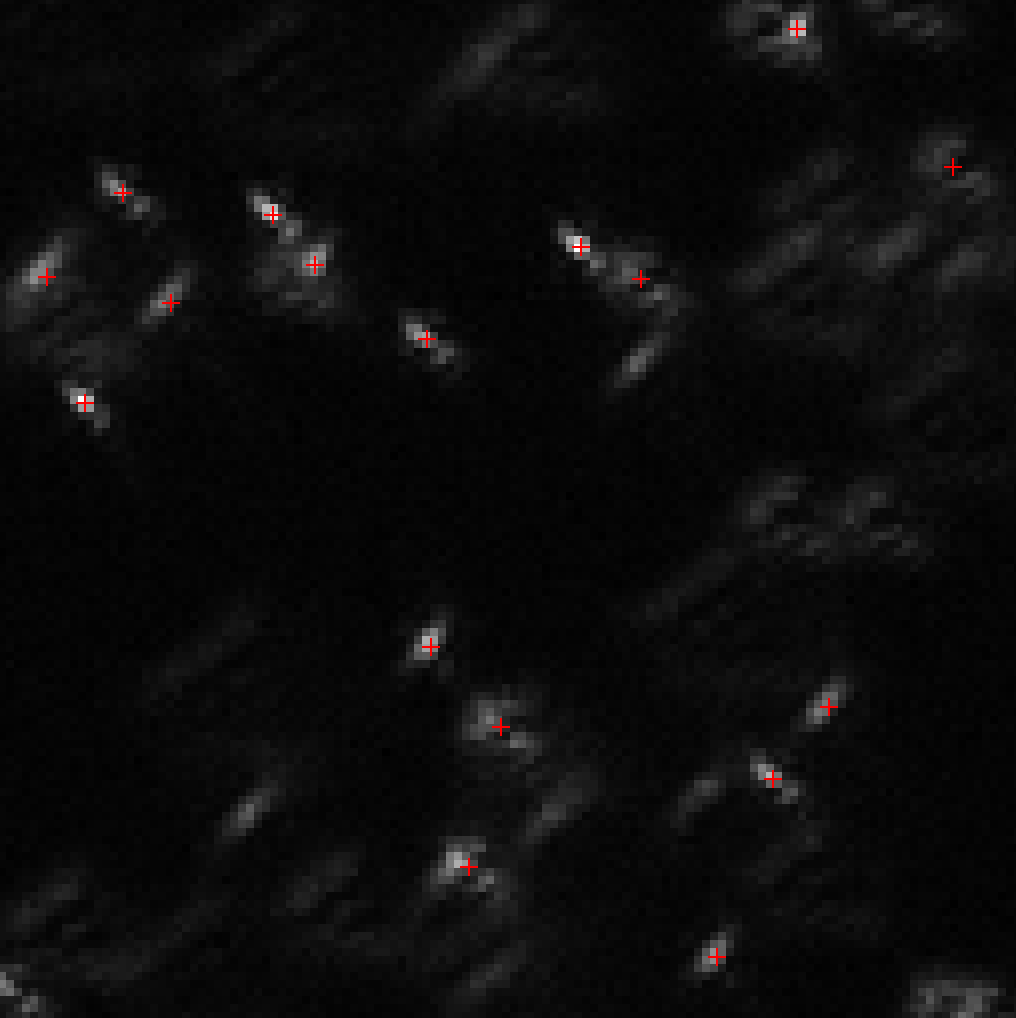
\includegraphics[width=\textwidth]{fig/X_loc.png}
            \caption{原始图像}
        \end{subfigure}
        \begin{subfigure}[b]{0.3\textwidth}
            \centering
            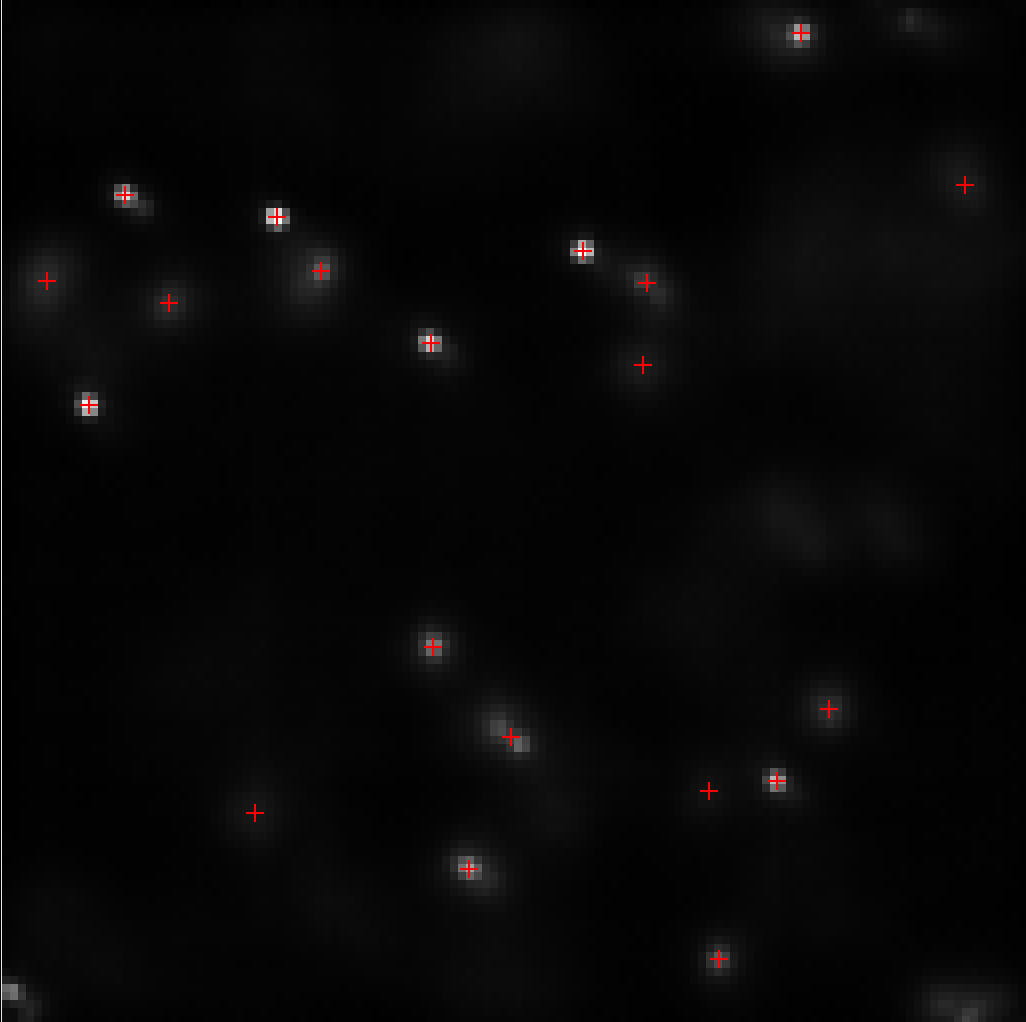
\includegraphics[width=\textwidth]{fig/y_hat_loc.png}
            \caption{去像差后}
        \end{subfigure}
        \begin{subfigure}[b]{0.3\textwidth}
            \centering
            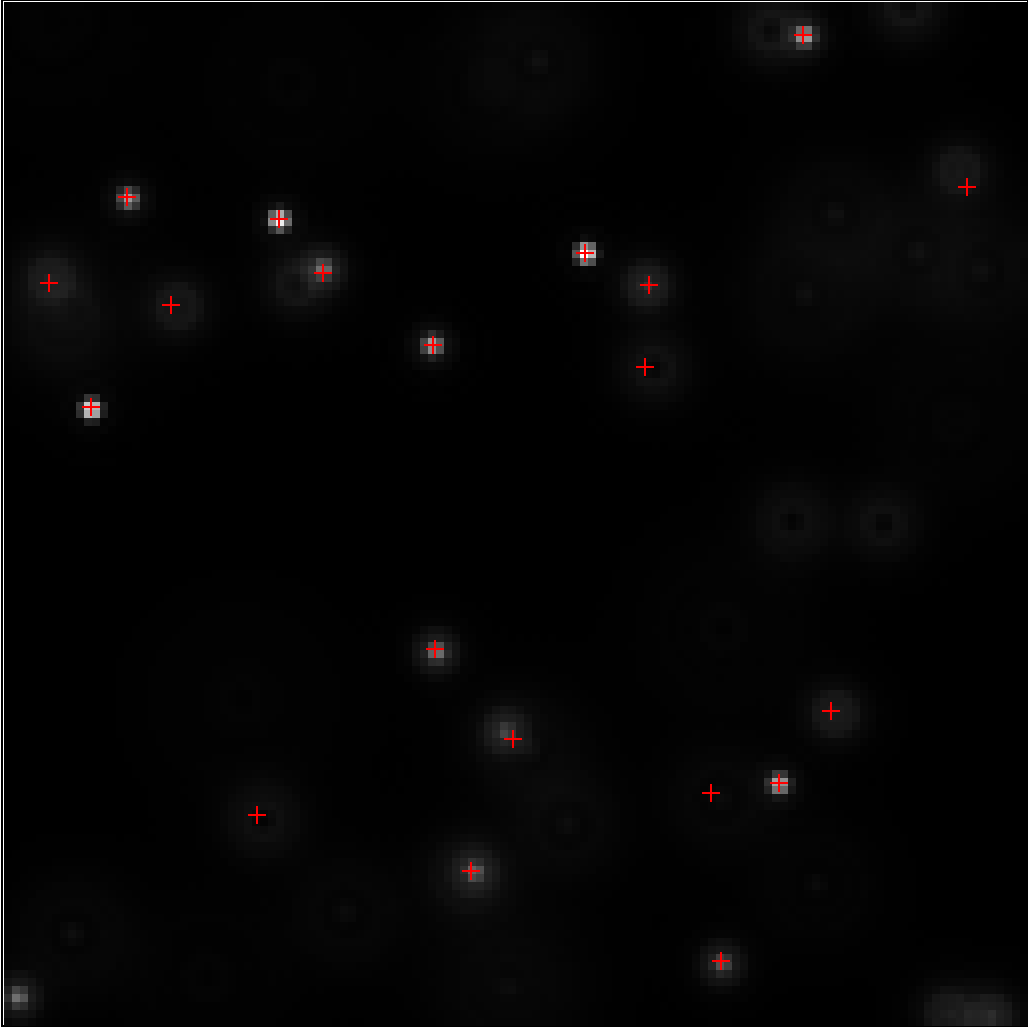
\includegraphics[width=\textwidth]{fig/y_loc.png}
            \caption{不含像差}
        \end{subfigure}
        \caption{ThunderSTORM定位示意}
        \label{Thm}
    \end{figure}
    \par 注意到，虽然测试选取了间接的方式，即由输出的图像再次经过定位算法，而非直接输出高精度坐标，该模型仍能够在一定程度上提升单分子定位的精度。这说明卷积神经网络能够较忠实地还原原始图像的信息，以改善其质量。


    \chapter{总结与展望}
    本文使用标量衍射理论对三维的点源扩散函数和像差进行了建模，并能够兼容不同的相位掩膜以进行点源扩散函数工程的研究。为了去除随机扰动的波前像差，使用含有13阶随机Zernike像差(即平均rms为0.65rad)的不同密度的随机点源图像作为训练集，搭建了编码-解码卷积网络以矫正像差。矫正后的图像表现出更好的质量，并在定位精度测试中优于未矫正图像。网络表现出一定的泛化能力(在未见过的、不同点源密度的数据集上正常运作)，这说明卷积网络具有捕捉细微结构并还原其信息的潜力。由于使用的训练集不包含特定物体的结构信息，该方法理论上可用于任何结构的单分子或高密度的成像。
    \par 碍于计算性能和时间，尚有不少研究可在未来进行。首先，本文使用了一个比较经典的架构；由于目前深度学习工具库的高度模块化，未来可尝试不同网络架构，如使用残差块来稳定模型、使用并行连接以包含不同尺寸的卷积块。其次，本文使用了低分辩图片作为输出。还可以尝试直接输出三维的PSF、或者二维的光瞳函数、抑或者直接输出定位位置。然后，本方法理论上亦可用于对含有相位掩膜的数据的去像差，以达到更高的三维定位精度。在数据处理和分析方面，还可以具体对含像差定位的信息矩阵进行计算、设计实验以验证实际上的定位精度。总体来说，本文提供了基本的实现上述功能的框架和基础，其中关键的matlab和python代码参见附录。


    \appendix
    \chapter*{附录A：信息矩阵的解析表达式}
    \phantomsection\addcontentsline{toc}{chapter}{附录A：信息矩阵的解析表达式}

    \par 对于2.3.1节所定义的模型，可通过卷积显式地写出每个像素的取值的概率密度分布：
    \begin{equation}
        p_{\theta, k}(z)=\frac{e^{-\nu_{\theta, k}}}{\sqrt{2 \pi} \sigma_{k}} \sum_{l=0}^{\infty} \frac{\nu_{\theta, k}^{l}}{l!} e^{\frac{-\left(z-l-\eta_{k}\right)^{2}}{2 \sigma_{k}^{2}}},\nu_{\theta, k}=s_{\theta,k}+\beta_{\theta,k}
        \label{distribution}
    \end{equation}
    因为每个像素的光子统计独立，对数似然函数可以写成：
    \begin{equation}
        l(\theta)=\ln \mathbb{P}\{X=x|\theta\}=\sum_k \ln \mathbb{P}\{X_k=x_k|\theta\}=\sum_k \ln p_{\theta, k}(x_k)
    \end{equation}
    求偏导：
    \begin{equation}
        \frac{\partial}{\partial\theta}\ln l(\theta)=\sum_k \frac{\partial}{\partial\theta} \ln p_{\theta, k}(x_k)
    \end{equation}
    求矩阵：
    \begin{equation}
        \ [\frac{\partial}{\partial\theta}\ln l(\theta)]^T[\frac{\partial}{\partial\theta}\ln l(\theta)]=\sum_k \sum_{k'}\ [\frac{\partial}{\partial\theta}\ln p_{\theta, k}(x_k)]^T[\frac{\partial}{\partial\theta}\ln p_{\theta, {k'}}(x_{k'})]
    \end{equation}
    取期望：
    \begin{equation}
        \textbf{I}(\theta)=\mathbb{E}\ [\frac{\partial}{\partial\theta}\ln l(\theta)]^T[\frac{\partial}{\partial\theta}\ln l(\theta)]=\sum_k \sum_{k'}\mathbb{E}\ [\frac{\partial}{\partial\theta}\ln p_{\theta, k}(x_k)]^T[\frac{\partial}{\partial\theta}\ln p_{\theta, {k'}}(x_{k'})]
    \end{equation}
    \begin{equation}
        [\textbf{I}(\theta)]_{ij}=\sum_k \sum_{k'}\ \mathbb{E}\ \{[\frac{\partial}{\partial\theta_i}\ln p_{\theta, k}(x_k)][\frac{\partial}{\partial\theta_j}\ln p_{\theta, {k'}}(x_{k'})]\} 
    \end{equation}
    交叉项($k\ne k’$)：
    \begin{equation}
        \begin{aligned}
            \int \int dx_k &dx_{k'} p_{\theta,k'}(x_k)p_{\theta,k}(x_{k'})\ \{[\frac{\partial}{\partial\theta_i}\ln p_{\theta, k}(x_k)][\frac{\partial}{\partial\theta_j}\ln p_{\theta, {k'}}(x_{k'})]\} \\  & =\int \int dx_k dx_{k'} \{[\frac{\partial}{\partial\theta_i} p_{\theta, k}(x_k)][\frac{\partial}{\partial\theta_j} p_{\theta, {k'}}(x_{k'})]\} \\ & =\frac{\partial}{\partial\theta_i}\frac{\partial}{\partial\theta_j}\int \int dx_k dx_{k'} p_{\theta, k}(x_k)p_{\theta, {k'}}(x_{k'})=0
        \end{aligned}
    \end{equation}
    因而可以去掉一个求和：
    \begin{equation}
        [\textbf{I}(\theta)]_{ij}=\sum_k \ \mathbb{E}\ \{[\frac{\partial}{\partial\theta_i}\ln p_{\theta, k}(x_k)][\frac{\partial}{\partial\theta_j}\ln p_{\theta, {k}}(x_{k})]\} 
    \end{equation}
    当待估计参数（位置，亮度等）仅仅通过影响像素的泊松分布系数来影响模型时（不含高斯噪声的估计），即可再将似然函数写成系数$\nu_{\theta, k}$的嵌套函数。这样上式用链式法则可拆分：
    \begin{equation}
        \begin{aligned}
            \relax[\textbf{I}(\theta)]_{ij} & =\sum_k \ \mathbb{E}\ \{[\frac{\partial \nu_{\theta, k}}{\partial\theta_i}\frac{\partial }{\partial\nu_{\theta, k}}\ln p_{\nu}(x_k)][\frac{\partial \nu_{\theta, k}}{\partial\theta_j}\frac{\partial }{\partial\nu_{\theta, k}}\ln p_{\nu}(x_k)]\} \\ & =\sum_k \  \frac{\partial \nu_{\theta, k}}{\partial\theta_i}\frac{\partial \nu_{\theta, k}}{\partial\theta_j}\mathbb{E}\  \{[\frac{\partial \ln p_{\nu}(x_k)}{\partial\nu_{\theta, k}}]^2\}
        \end{aligned}
    \end{equation}
    \begin{equation}
        \textbf{I}(\theta)=\sum_k (\frac{\partial \nu_{\theta, k}}{\partial\theta})^T(\frac{\partial \nu_{\theta, k}}{\partial\theta})\mathbb{E}\  \{[\frac{\partial \ln p_{\nu}(x_k)}{\partial\nu_{\theta, k}}]^2\}
    \end{equation}
    \par 注意在该式中，若固定PSF模型，则单个像素所包含的参数信息取决于一个标量的期望项。这一项显然是和传感器及背景噪声相关的(detector dependent)。代入式(\ref{distribution})得：
    \begin{equation}
        \begin{aligned}\mathbf{I}(\theta)= & \sum_{k=1}^{K}\left(\frac{\partial \nu_{\theta, k}}{\partial \theta}\right)^{T}\left(\frac{\partial \nu_{\theta, k}}{\partial \theta}\right) \\& \times\left(\int_{-\infty}^{\infty} \frac{\left(\frac{e^{-v_{\theta, k}}}{\sqrt{2 \pi} \sigma_{k}} \sum_{l=1}^{\infty} \frac{\nu_{\theta, k}^{l-1}}{(l-1)!} e^{\frac{-\left(z-l-\eta_{k}\right)^{2}}{2 \sigma_{k}^{2}}}\right)^{2}}{p_{\theta, k}(z)} \mathrm{d} z-1\right),\end{aligned}
    \end{equation}
    
    \chapter*{附录B：部分关键问题的matlab和python代码实现}
    \phantomsection\addcontentsline{toc}{chapter}{附录B：部分关键问题的matlab和python实现}
    \subsection*{带有相位掩膜和像差的光瞳函数}
    首先需要根据需要确定相位掩膜的具体形式，将其整合在一个二维、具有圆形形状的矩阵pupilFun中。如2.2节所述，该矩阵代表频率空间，因而其尺寸需要和采样精度匹配；同时其圆形直径由式(\ref{pupil_r})决定。在本文中统一使用6倍(UpSampling)于传感器像素数量的格点以保证足够的理论计算精度(xSizeUp)。则pupilFun的数据应具有模长和相位、代表强度和相位的调制。则根据Zernike函数，传入极坐标和随机生成的系数，可以算出每一点对应的相位差(phi)。其即代表了随机的波前像差，通过角度部分整合进光瞳函数中(pupilFunAbe)。其关键逻辑见如下matlab代码：

    \begin{lstlisting}[language=Matlab]
    % Generate the original pupil function
    [r, theta, idx] =  def_pupilcoor(xSizeUp, xPixelSizeUp,...
         lambda, NA); % convert into polar coordinates
    r0 = r(idx); 
    theta0 = theta(idx);
    pupilMask = zeros(xSizeUp, xSizeUp, 'single');
    pupilMask(idx) = 1;

    % Generate random zernike coefficients
    coeffs = gen_zern_coeffs(pIn,aValue,zernType);
    coeffs = wavenumber * coeffs; % Make into wavenumber units

    % Generate aberrated pupil function
    phi = zeros(xSizeUp, xSizeUp, 'single');
    phi(idx) = create_wavefront(zernIndex, coeffs, r0, theta0); 
    pupilFunAbe = pupilFun.*exp(1i*phi);
    \end{lstlisting}
    
    注意此处代码使用的是默认圆形的原始光瞳函数，如需要生成带掩膜的光瞳只需要乘以对应的掩膜形式即可。

    \subsection*{从光瞳函数到含像差的单分子图像}
    模拟得到含有像差信息的光瞳函数后，我们需要引入z轴参量生成三维的点源扩散函数。其使用的公式见\ref{z_pupil}，具体而言我们在人为定义的z轴格点上计算PSF，本文中使用的z轴分辨率和xy轴相同，跨度为4.16微米，matlab代码如下：

    \begin{lstlisting}[language=Matlab]
    function PSF3d = gen_PSF3D(xPixelSize, xSize, ...
        zPixelSize, zSize, lambda, RI, pupilFun, pupilMask)
    % Generate 3D PSF based on pupil function
    dConst = defocus_wavefront(xPixelSize, xSize, ...
        lambda, RI, pupilMask); 
    PSF3d = zeros(xSize, xSize, zSize, 'single');
    Soz = (zSize+1)/2; 
    for i = 1:zSize
        zPos = (i - Soz) * zPixelSize;
        pupilFun2D = pupilFun .*exp(1i*zPos*dConst);
        prf = fftshift(ifft2(ifftshift(pupilFun2D)));
        PSF3d(:,:,i) = abs(prf).^2;
    end
    PSF3d = PSF3d/max(PSF3d(:)); % normalization
    \end{lstlisting}
    
    随机生成的点源以其坐标储存，考虑到计算复杂度，只生成跨度4.16微米范围内的点源。然后根据点源位置不同选取上文算出的3D PSF的截面作为其2D PSF，通过线性叠加即可得到模拟的单分子点源。其实现matlab代码如下：

    \begin{lstlisting}[language=Matlab]
    function pointsBlur2D = gen_blurred2D(xSizeUp, ...
        zSizeUp,positions,emitterNumber,PSF3d)

    pointsBlur2D = zeros(xSizeUp, xSizeUp, 'single');
    PSF3d = PSF3d/sum(PSF3d(:,:,10), "all");

    for i = 1:emitterNumber
        x = positions(i,1);
        y = positions(i,2);
        z = positions(i,3);
        N = positions(i,4); 
        x_start = max(1, x+1);
        x_end   = min(xSizeUp, x + xSizeUp);
        y_start = max(1, y+1);
        y_end   = min(xSizeUp, y + xSizeUp);
        z_index = zSizeUp/2 + 1 - z; 
        z_index = max(1, min(z_index, zSizeUp)); % 防止超界

        psf_x_start = 1 + (x_start - (x+1));
        psf_x_end   = xSizeUp - ((x + xSizeUp) - x_end);
        psf_y_start = 1 + (y_start - (y+1));
        psf_y_end   = xSizeUp - ((y + xSizeUp) - y_end);

        pointsBlur2D(x_start:x_end, y_start:y_end) = ...
            pointsBlur2D(x_start:x_end, y_start:y_end) + ...
            PSF3d(psf_x_start:psf_x_end, psf_y_start: ...
            psf_y_end, z_index) * N; % 累加 PSF 到 2D 平面
    end 
    \end{lstlisting}

    注意3D PSF按每层总和作了归一化，以保证发出光子数为N的点源在像面上总是加和为N（即完全截获）。点源亮度N设为均值6000、方差500的正态分布；点源密度可改变，其模拟和模型结果见第三章。此后再按每个像素添加散粒噪声、泊松噪声(lambda=5)和高斯噪声(mean = 2; std=0.2)即可。最后得到的图像需要按之前作的UpSampling比例下采样到真实传感器的密度。其点源示意图图\ref{points_3d}
    \begin{figure}[h] 
        \centering
        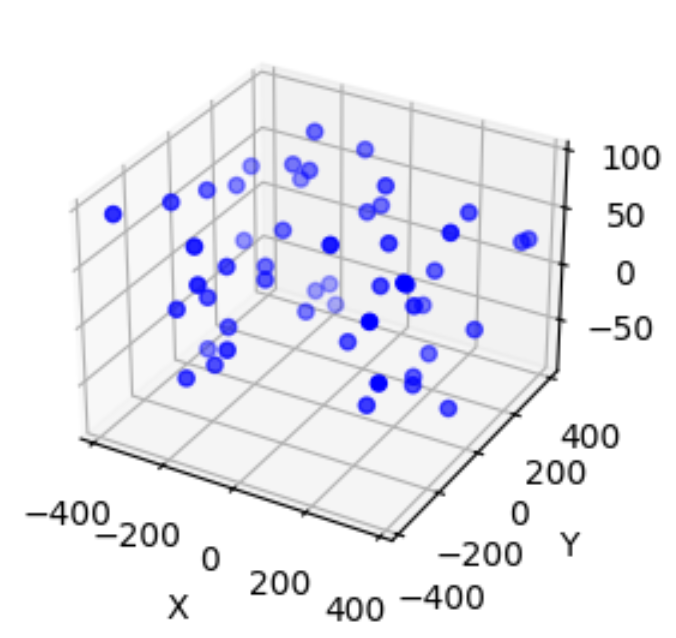
\includegraphics[width=0.7\textwidth]{fig/points_3d.png}
        \caption{三维中间中随机生成的点源（低密度）}
        \label{points_3d}
    \end{figure}

    \subsection*{基于pytorch的编码解码器网络}
    pytorch已经集成了大部分训练网络需要的工具。本文使用的编码-解码器网络架构类定义如下：

    \begin{lstlisting}[language=Python,breaklines=true]
    class EncoderDecoder(nn.Module):
    def __init__(self):
        super(EncoderDecoder, self).__init__()
        self.encoder = nn.Sequential(
            nn.Conv2d(1, 16, kernel_size=7, stride=2, padding=3),
            nn.BatchNorm2d(16),
            nn.ReLU(),
            nn.Conv2d(16, 64, kernel_size=5, stride=2, padding=2),
            nn.BatchNorm2d(64),
            nn.ReLU(),
            nn.Conv2d(64, 128, kernel_size=5, stride=2, padding=2),
            nn.BatchNorm2d(128),
            nn.ReLU(),
            nn.Conv2d(128, 512, kernel_size=5, padding=2),
            nn.BatchNorm2d(512),
            nn.ReLU(),
        )
        self.decoder = nn.Sequential(
            nn.ConvTranspose2d(512, 128, kernel_size=4, stride=2, padding=1),
            nn.BatchNorm2d(128),
            nn.ReLU(),
            nn.ConvTranspose2d(128, 64, kernel_size=4, stride=2, padding=1),
            nn.BatchNorm2d(64),
            nn.ReLU(),
            nn.ConvTranspose2d(64, 1, kernel_size=4, stride=2, padding=1),
            nn.Sigmoid()
        )
    def forward(self, x):
        x = self.encoder(x)
        x = self.decoder(x)
        return x
    \end{lstlisting}

    L1L2损失函数定义如下：

    \begin{lstlisting}[language=Python,breaklines=true]
    class L1L2Loss(nn.Module):
    def __init__(self, alpha=0.6):  # α 控制 L1 和 L2 的比例
        super(L1L2Loss, self).__init__()
        self.alpha = alpha
        self.l1_loss = torch.nn.SmoothL1Loss()
        self.l2_loss = nn.MSELoss()
        self.ssim = ssim

    def forward(self, y_pred, y_true):
        l1 = self.l1_loss(y_pred, y_true) * 100 * 100 # for convinence of visualization
        l2 = self.l2_loss(y_pred, y_true) * 100 * 100
        # ssim = 1 - self.ssim(y_pred, y_true, data_range=1.0) 
        return  self.alpha * l1 + (1 - self.alpha) * l2
    \end{lstlisting}

    其他组件均使用pytorch常规组件(优化器=torch.optim.Adam，初始化=torch.nn.init.kaiming\_normal\_)，不再赘述。

    \phantomsection\addcontentsline{toc}{chapter}{参考文献}
    \bibliography{../MyLibrary}
    \bibliographystyle{ieeetr}

    \chapter*{致谢}
    \phantomsection\addcontentsline{toc}{chapter}{致谢}
    首先我要感谢张云翔老师，这篇论文的想法和完成离不开他几乎每周一对一的解惑和指导、还有光学平台上手把手式的教导。自去年暑假开始自学光学的基础内容，我花了一个多学期掌握了光学基本的知识。尽管Hecht的\textit{Optics}写的非常难懂，好在有梁铨延编著的《物理光学》帮助我理解了光的单界面行为和干涉的基本原理。杨葭隼先生翻译的Born和Wolfmann的名著\textit{Principles of Optics}行文流畅，为未系统学习电动力学的我打开了理解光学的新大门。
    \par 寒假的时间里，Goodmann的《傅立叶光学》帮助我理解了复杂的衍射现象，也意料之外地用上了去年修读的信号处理的课程的知识。多亏了这些基础，我才能在程序上一步步实现一些衍射成像信号的模拟。尽管去年的课上没怎么听明白，但是清华大学张颢老师的《数字信号处理》视频帮助我深刻地理解了采样定理和傅立叶变换，构成了本文得以完成的知识基础。
    \par 关于神经网络的实践实现主要依靠李沐大神的《动手学深度学习》，也需要感谢上学期陈惠老师主持的《ai在分析化学中的应用》让我拓展了ai相关的视野和能力。
    \par 总之，作为我自选自研的课题，这篇论文的工作显然还是很初步和稚嫩的，但也确实锻炼到相关的能力。光学的概念似乎也确实只有亲自模拟过才能理解其直观，希望本文的经验能在未来发挥作用。

\end{document}